\documentclass[pdflatex,sn-mathphys-num]{sn-jnl}

\usepackage{graphicx}
\usepackage{multirow}
\usepackage{amsmath,amssymb,amsfonts}
\usepackage{amsthm}
\usepackage{mathrsfs}
\usepackage[title]{appendix}
\usepackage{xcolor}
\usepackage{textcomp}
\usepackage{manyfoot}
\usepackage{booktabs}
\usepackage{makecell}
\usepackage{url}
\usepackage{listings}

\theoremstyle{thmstyleone}
\newtheorem{theorem}{Theorem}
\newtheorem{proposition}[theorem]{Proposition}

\theoremstyle{thmstyletwo}
\newtheorem{example}{Example}
\newtheorem{remark}{Remark}

\theoremstyle{thmstylethree}
\newtheorem{definition}{Definition}

\raggedbottom

\begin{document}

\title[Integrating Blockchain and IPFS for Ex-Post Auditing in FL]{Integrating Blockchain and IPFS for Traceability, Integrity, and Ex-Post Auditing in Federated Learning}

\author*[1]{\fnm{David Piotr} \sur{Znojek}}\email{dawidznojek@gmail.com}

\author[1]{\fnm{Francisco A.} \sur{Pujol}}\email{fpujol@ua.es}

\affil*[1]{\orgdiv{Department of Computer Technology and Computation}, \orgname{University of Alicante}, \orgaddress{\street{Carretera de San Vicente del Raspeig s/n}, \city{San Vicente del Raspeig}, \postcode{03690}, \state{Alicante}, \country{Spain}}}

\abstract{Federated learning preserves edge data privacy but lacks intrinsic mechanisms to verify participant contributions, exposing distributed systems to poisoning attacks. This paper presents a hybrid architecture integrating a permissioned Ethereum Virtual Machine blockchain (Hyperledger Besu) with off-chain content-addressable storage (InterPlanetary File System). A smart contract coordinates bidirectional cross-verification using cryptographic commitments of model weights, complemented by an independent ex-post audit protocol to mathematically verify aggregation fidelity. Evaluated on a distributed testbed across 15 executions (450 rounds) classifying vehicular road events, the blockchain layer adds an overhead of only 9.5\% (6.34 seconds per round) with deterministic, invariant gas consumption. In-transit tampering is intercepted within 149 milliseconds, and ex-post auditing reconstructs canonical aggregation in 0.34 seconds with exact mathematical correspondence. These findings confirm that the operational cost of decentralization, immutability, and non-repudiation is thoroughly viable and affordable compared to the critical auditability guarantees obtained.}

\keywords{Federated learning, Blockchain, IPFS, Traceability, Ex-post auditing, Byzantine fault tolerance}

\maketitle

% !TeX root = ../main.tex
\section{Introduction}
\label{sec:introduccion}

The rapid proliferation of Artificial Intelligence (AI) and Machine Learning (ML) has transformed critical sectors, including healthcare, finance, and intelligent transportation systems. However, training high-capacity models requires massive volumes of data, which frequently contain sensitive or proprietary information, such as high-resolution geolocation traces, user behavior patterns, or biometric identifiers. Under traditional centralized paradigms, gathering raw data into a single repository introduces severe privacy vulnerabilities, regulatory compliance challenges (such as the GDPR), and substantial computational and communication bottlenecks.

Federated Learning (FL)~\cite{mcmahan2017federated} emerged as a decentralized paradigm where distributed edge nodes iteratively train local model instances on their private datasets, transmitting only updated weight vectors or gradients to a central coordinator. Although FL avoids direct exposure of raw data, it introduces a structural security challenge: the absence of inherent trust among participating entities. In an unsupervised, distributed environment, malicious actors or compromised edge nodes can launch data poisoning, model poisoning, or backdoor insertion attacks~\cite{bagdasaryan2020backdoor} by submitting manipulated model updates. For instance, in Connected and Autonomous Vehicles (CAVs)~\cite{chellapandi2024federated}, a subtle, coordinated perturbation in model parameters could lead the global classifier to misidentify critical road hazards or traffic signals (e.g., failing to detect a STOP sign), yielding catastrophic consequences.

To address these vulnerabilities, integrating Blockchain technology with Federated Learning (BCFL)~\cite{qu2022blockchain} provides an immutable, decentralized, and verifiable ledger~\cite{nakamoto2008bitcoin, zheng2018blockchain}. By embedding a distributed ledger into the federated training workflow, parameter updates, aggregation rounds, and participant identities are cryptographically anchored via smart contracts, establishing an end-to-end, auditable, and non-repudiable record of all training contributions.

Nevertheless, this convergence introduces a critical system-level trade-off: \textbf{security versus operational performance}. While blockchain provides immutability and Byzantine fault tolerance, it inherently introduces network latency, consensus delays, transaction confirmation overhead, and additional computational resource demands. In mission-critical edge computing environments~\cite{liu2019edge}, it is essential to answer a fundamental question: \textit{what temporal and computational overhead must be incurred to achieve a more auditable and tamper-resistant federated training?}

\subsection{Motivation and Prior Work}
This work builds upon and extends two research lines conducted at the University of Alicante:
\begin{enumerate}
    \item \textbf{Real-time vehicular event verification}~\cite{pujol2024blockchain}: demonstrated the feasibility of a private Hyperledger Besu network operating under Istanbul Byzantine Fault Tolerant (IBFT 2.0) consensus to log vehicular traffic alerts with sub-second latencies (0.32 to 0.82~s), outperforming human reaction times.
    \item \textbf{FL-Blockchain architectural framework}~\cite{cloudlabaia_flblockchain}: conceptually proposed using smart contracts to record cryptographic hashes of model weights at each federated round.
\end{enumerate}

The present study formally designs, implements, and empirically validates the convergence of these proposals on a physical distributed testbed, evaluating both cryptographic integrity guarantees and temporal system performance.

\subsection{Main Contributions}
The main contributions of this paper are summarized as follows:
\begin{itemize}
    \item \textbf{Hybrid architecture design}: We formulate an end-to-end framework coupling a permissioned Hyperledger Besu blockchain network with the Flower federated learning framework~\cite{beutel2020flower} and off-chain, content-addressable distributed storage via IPFS.
    \item \textbf{Traceability and integrity via smart contracts}: We design and deploy a Solidity smart contract that orchestrates bidirectional cross-verification of models through content identifiers (IPFS CIDs, encapsulating SHA-256 multihashes of serialized artifacts), immutably anchoring each participant's contribution and the aggregated global model per round.
    \item \textbf{Empirical adversarial validation}: We subject the platform to deliberate weight-corruption attack vectors (both in-transit tampering from an untrusted server and unauthorized/poisoning injections from clients), validating that the bidirectional verification protocol deterministically intercepts integrity discrepancies and rogue models with low response latencies (31 to 149~ms).
    \item \textbf{Ex-post audit protocol and mathematical FedAvg verification}: We develop and evaluate an independent, off-band audit protocol enabling any consortium participant or third-party auditor to retrospectively verify aggregator fidelity. We demonstrate the ability to mathematically reconstruct canonical FedAvg aggregation directly from immutable commitments stored on Besu and IPFS, achieving exact numerical correspondence ($\Delta = 0$, CID match) in $0.34$~s, while detecting unauthorized parameter deviations in $0.18$~s.
    \item \textbf{Quantitative infrastructure benchmarking}: We deploy a convolutional traffic event classifier to serve as a representative workload for extracting reproducible system-level metrics (temporal overhead, EVM gas consumption, and validator scaling), delimiting hyperparameter and model optimization as future work.
    \item \textbf{Operational feasibility analysis}: We analytically resolve the latency-versus-security dilemma, characterizing the operational regimes where blockchain logging overhead is thoroughly justified compared to unverified setups.
\end{itemize}

To facilitate scientific reproducibility and technology transfer, the complete framework source code, Solidity smart contracts, Hyperledger Besu Docker Compose deployment templates, and experimental evaluation scripts are openly available on GitHub: \url{https://github.com/dpz6-ua/Blockchain_ML}.

\subsection{Paper Organization}
The remainder of this paper is structured as follows: Section~\ref{sec:estado_arte} reviews related work and theoretical foundations of Blockchain and Federated Learning. Section~\ref{sec:arquitectura} details the proposed architecture and smart contract design. Section~\ref{sec:implementacion} describes the experimental testbed and dataset. Section~\ref{sec:evaluacion} presents and discusses empirical performance, scalability, and security validation results. Finally, Section~\ref{sec:conclusiones} concludes the paper and outlines future research directions.

% !TeX root = ../main.tex
\section{Theoretical Foundations and Related Work}
\label{sec:estado_arte}

The proposed architecture converges three fundamental technological pillars: permissioned distributed ledgers with Byzantine Fault Tolerant (BFT) consensus, content-addressable distributed storage, and federated learning. Below, we synthesize their theoretical foundations and examine the critical limitations identified in the related literature.

\subsection{Permissioned Blockchain and IBFT 2.0 Consensus}
A blockchain is an immutable, distributed data structure where transactions are bundled into cryptographically linked blocks using collision-resistant hash functions (such as SHA-256)~\cite{nist2015sha, zheng2018blockchain}. Unlike public (permissionless) networks such as Bitcoin or Ethereum Mainnet, which suffer from high transaction latency and volatile monetary fees, industrial consortia predominantly adopt permissioned networks compatible with the Ethereum Virtual Machine (EVM)~\cite{buterin2014ethereum}, such as Hyperledger Besu~\cite{besu_docs}.

In these environments, compute-intensive (Proof-of-Work, PoW) or stake-based (Proof-of-Stake, PoS) mechanisms are replaced by Byzantine Fault Tolerant consensus algorithms. The \textbf{IBFT 2.0} (\textit{Istanbul Byzantine Fault Tolerant}) protocol~\cite{moniz2020istanbul} organizes consensus around a predefined set of validator nodes that alternate the proposer role in a round-robin schedule. A proposed block is appended to the ledger only after a three-phase voting process (pre-prepare, prepare, commit) signed by a two-thirds supermajority of validators:
\begin{equation}
n \ge 3f + 1
\end{equation}
where $n$ denotes the total number of validator nodes and $f$ represents the maximum number of tolerated faulty or Byzantine participants.

IBFT 2.0 provides a pivotal advantage over probabilistic consensus models: \textbf{immediate deterministic finality}. Because the chain does not experience probabilistic forks, once a training round commitment or model update is sealed within a block, it achieves immediate finality and permanent immutability on the ledger. Furthermore, while the transaction gas price is set to zero in private consortia to eliminate monetary friction, the computational metric of \textit{gas used}~\cite{ethereum_gas} remains an objective, deterministic measure of execution and storage overhead imposed on the EVM.

\subsection{Off-Chain Distributed Storage (IPFS)}
Directly persisting deep neural network parameters on a blockchain ledger is technically infeasible due to model artifact sizes (ranging from dozens to hundreds of megabytes), which would rapidly trigger severe EVM state bloat and demand prohibitive gas execution limits.

To overcome this bottleneck, we adopt the paradigm of \textbf{off-chain storage with on-chain commitment} utilizing the InterPlanetary File System (IPFS)~\cite{benet2014ipfs, daniel2022ipfs}. IPFS operates over a peer-to-peer (P2P) network based on content addressing and Merkle Directed Acyclic Graph (Merkle DAG) structures~\cite{daniel2022ipfs, trautwein2022design}: files are partitioned into immutable chunks and addressed through a unique Content Identifier (CID) derived directly from their cryptographic hash. The global-scale empirical and architectural evaluation conducted by Trautwein et al.~\cite{trautwein2022design} demonstrates that its block-exchange protocol (Bitswap) and distributed hash table (Kademlia DHT) achieve decentralized content routing with minimal overhead. By decoupling weight artifact storage to IPFS and recording only the content identifier (IPFS CIDv0, encapsulating the SHA-256 multihash of the serialized weights) within the smart contract~\cite{zhao2021privacy}, subsequent downloads can be validated against the immutable ledger. This provides data deduplication, formal integrity verification, and distributed access at negligible on-chain execution cost, provided that operational availability and persistence are backed by content pinning or dedicated IPFS nodes.

\subsection{Federated Learning and the FedAvg Algorithm}
Federated Learning (FL)~\cite{mcmahan2017federated} preserves data privacy by decoupling local model optimization from central parameter aggregation. Among federated consensus mechanisms, \textbf{FedAvg} (\textit{Federated Averaging}) serves as the foundational standard. At each communication round $t$, the aggregation coordinator broadcasts the current global weight vector $w^{(t)}$ to a selected set of $K$ edge clients. Each client trains the model on its private partition $\mathcal{D}_k$ by minimizing a local loss function, yielding updated local parameter weights $w_k^{(t)}$. The server then computes the consolidated global model as a sample-weighted average based on local sample counts $n_k$:
\begin{equation}
w^{(t+1)} = \sum_{k=1}^{K} \frac{n_k}{n} \, w_k^{(t)}, \quad \text{where } n = \sum_{k=1}^{K} n_k
\end{equation}

The \textbf{Flower} framework~\cite{beutel2020flower} offers a modular, efficient infrastructure to coordinate this federated lifecycle via bidirectional remote procedure calls over gRPC.

\begin{sidewaystable}
\caption{Qualitative and architectural comparison against relevant Blockchain-FL and robustness frameworks in the literature.}\label{tab:estado_arte}
\footnotesize
\setlength{\tabcolsep}{3.5pt}
\renewcommand{\arraystretch}{1.15}
\begin{tabular*}{\textheight}{@{\extracolsep\fill}lccccc}
\toprule
\textbf{Proposal / Framework} & \makecell{\textbf{Blockchain}\\\textbf{Consensus}} & \makecell{\textbf{Model}\\\textbf{Storage}} & \makecell{\textbf{Verification}\\\textbf{Protocol}} & \makecell{\textbf{Transactional}\\\textbf{Cost}} & \makecell{\textbf{Fault}\\\textbf{Tolerance}} \\
\midrule
\makecell[l]{Krum\\(Blanchard et al.)~\cite{blanchard2017byzantine}} & \makecell{No Blockchain\\(Centralized)} & \makecell{Central server\\(SPOF)} & \makecell{Geometric selection\\($L_2$)} & \makecell{None\\(No ledger)} & \makecell{Strict Byzantine\\($f < \frac{N-2}{2}$)} \\ \midrule
\makecell[l]{BlockFL\\(Kim et al.)~\cite{kim2019blockfl}} & \makecell{PoW\\(Slow / Inefficient)} & \makecell{On-Chain\\(Storage bottleneck)} & Unidirectional & \makecell{Volatile\\cryptocurrency} & \makecell{Probabilistic\\($< 50\%$)} \\ \midrule
\makecell[l]{DeepChain\\(Weng et al.)~\cite{weng2021deepchain}} & \makecell{PoW / PBFT\\with incentives} & \makecell{On-Chain\\(Encrypted gradients)} & \makecell{Homomorphic Enc.\\+ MACs} & \makecell{Severe (Massive\\on-chain ciphertext)} & \makecell{Formal Byzantine\\($f < N/3$)} \\ \midrule
\makecell[l]{AV-BFL\\(Pokhrel \& Choi)~\cite{pokhrel2020federated}} & \makecell{Adaptive PoW /\\DPoS} & \makecell{On-Chain\\at RSUs} & \makecell{Base station\\verification} & \makecell{Wireless\\retransmissions} & \makecell{Constrained by\\vehicular channel} \\ \midrule
\makecell[l]{H-BCFL\\(Chai et al.)~\cite{chai2021hierarchical}} & \makecell{Hierarchical DPoS\\at RSUs} & \makecell{On-Chain at\\base stations} & \makecell{Reputation and\\knowledge audit} & \makecell{Edge clustering\\overhead} & \makecell{Dependent on\\RSU reliability} \\ \midrule
\makecell[l]{B5G-FL\\(Lu et al.)~\cite{lu2020blockchain}} & \makecell{Permissioned\\(PBFT / BFT)} & \makecell{On-Chain at\\base stations} & \makecell{Base station\\consensus} & \makecell{DRL\\optimization} & \makecell{Formal Byzantine\\($f < N/3$)} \\ \midrule
\makecell[l]{Vehicular BFL\\(Pujol et al.)~\cite{pujol2024blockchain}} & \makecell{IBFT 2.0\\(Permissioned)} & \makecell{IoT alert\\logging} & \makecell{Traffic\\monitoring} & \makecell{Commercial\\gas-free} & \makecell{Formal Byzantine\\($N \ge 3f + 1$)} \\ \midrule
\makecell[l]{BCFL-Ref\\(Goh et al.)~\cite{goh2023blockchain}} & \makecell{PoW / PoA\\(Ethereum)} & \makecell{Hybrid Off-Chain\\(IPFS)} & \makecell{Unidirectional\\(No cross-verification)} & \makecell{Variable gas\\(Public/private net)} & \makecell{Formal Byzantine\\(Ethereum consensus)} \\ \midrule
\makecell[l]{\textbf{Our Architecture}} & \makecell{\textbf{QBFT / IBFT 2.0}\\\textbf{(Besu)}} & \makecell{\textbf{Content-addressable}\\\textbf{storage (IPFS)}} & \makecell{\textbf{Bidirectional Cross-Verif.}\\\textbf{+ Ex-Post Audit}} & \makecell{\textbf{Stable gas per}\\\textbf{transaction}} & \makecell{\textbf{Formal Byzantine}\\\textbf{($f=1 \to 2$)}} \\
\bottomrule
\end{tabular*}
\end{sidewaystable}

\subsection{Vulnerabilities in FL and Related Work}
Despite privacy advantages, conventional Federated Learning frameworks suffer from intrinsic vulnerabilities classified in recent security taxonomies and surveys~\cite{bouacida2021vulnerabilities, jere2021taxonomy, qu2022blockchain}:
\begin{enumerate}
    \item \textbf{Central server as a single point of failure and trust}: Existing frameworks offer no native mechanism to verify whether the central coordinator faithfully executes FedAvg or intentionally injects malicious biases into the global parameter vector $w^{(t+1)}$.
    \item \textbf{Poisoning attacks and lack of non-repudiation}: Compromised edge clients can execute model poisoning or inject stealthy backdoors~\cite{bagdasaryan2020backdoor}. In the absence of an immutable, non-repudiable log linking cryptographic identities to parameter digests, attributing malicious updates or auditing the history of compromised models becomes impossible.
\end{enumerate}

To address these vulnerabilities, researchers have increasingly investigated the hybridization of Blockchain and Federated Learning (BCFL)~\cite{qu2022blockchain}. However, designing practical architectures for Connected and Autonomous Vehicles (CAVs/IoV) involves four fundamental engineering trade-offs:

\textbf{1. On-Chain vs. Hybrid Off-Chain Storage and Computation:} Pioneer architectures such as BlockFL~\cite{kim2019blockfl} proposed exchanging full weight matrices directly over the blockchain ledger. Similarly, DeepChain~\cite{weng2021deepchain} integrated decentralized auditing and economic incentives with homomorphic encryption (HE) of gradients, incurring extreme computational and on-chain storage bottlenecks. Other designs, such as FLChain~\cite{bao2019flchain}, explored decentralized auditing using distributed Bloom filters, finding that serializing massive parameter tensors within blockchain transactions triggers acute EVM state bloat and degrades throughput. Consequently, the hybrid paradigm—leveraging content-addressable off-chain storage via IPFS anchored to on-chain cryptographic hashes~\cite{zhao2021privacy, goh2023blockchain}—represents an efficient approach to prevent ledger bloat while ensuring scalability in distributed deployments.

\textbf{2. Consensus Mechanisms and Latency in Wireless and Vehicular Networks:} In autonomous driving and edge computing (5G and beyond), communication latency and resource constraints are primary bottlenecks~\cite{pokhrel2020federated, lu2020blockchain}. Proof-of-Work (PoW) protocols introduce multi-minute confirmation delays and probabilistic forks that are intolerable in safety-critical vehicular systems~\cite{kim2019blockfl}. To optimize resource allocation and model convergence in cellular edge networks, Lu et al.~\cite{lu2020blockchain} formulated a base-station permissioned blockchain utilizing deep reinforcement learning (DRL) for dynamic bandwidth allocation, while Pokhrel and Choi~\cite{pokhrel2020federated} developed analytical models characterizing vehicular wireless channel dynamics on consensus delay. In the Internet of Vehicles (IoV), Chai et al.~\cite{chai2021hierarchical} proposed a hierarchical architecture offloading aggregation and DPoS consensus to Roadside Units (RSUs), Qi et al.~\cite{qi2021privacy} combined permissioned blockchain with differential privacy for traffic flow prediction, and Abou El Houda et al.~\cite{abouelhouda2024blockchain} devised collaborative intrusion detection schemes via BCFL. However, these frameworks depend heavily on the continuous availability and synchronization of fixed roadside infrastructure. Rather than relying on high-latency public networks or foregoing Byzantine fault tolerance, permissioned consortia running IBFT 2.0 / QBFT such as Hyperledger Besu~\cite{pujol2024blockchain} provide immediate deterministic finality and rigorous Byzantine resilience ($N \ge 3f + 1$) without monetary fee fluctuations.

\textbf{3. Cryptographic Integrity vs. Statistical Robustness:} Two complementary defensive tiers exist in federated learning security~\cite{bouacida2021vulnerabilities, jere2021taxonomy}. On the one hand, decentralized immutable ledgers provide formal guarantees regarding in-transit artifact integrity, sender authentication, and non-repudiation. On the other hand, if a participating client deliberately manipulates its local training data while legitimately signing and registering the resulting weights on-chain (\textit{data/model poisoning}), statistical aggregation defenses against anomalous gradients are essential. Literature has explored geometric filtering such as Krum~\cite{blanchard2017byzantine}, coordinate-wise trimming including Trimmed-Mean and Median~\cite{yin2018byzantine}, and hybrid defenses against complex collusions such as Bulyan~\cite{mhamdi2018hidden}. Similarly, FLTrust~\cite{cao2021fltrust} introduced trust bootstrapping by evaluating angular parameter similarity against a root dataset maintained by the coordinator. These two layers are complementary: on-chain non-repudiation unambiguously attributes each parameter update to a specific cryptographic identity, enabling post-facto forensic auditing and smart-contract-coordinated slashing once statistical anomalies are identified.

\textbf{4. Aggregator Accountability (Black-Box Aggregation vs. Ex-Post Auditing):} In verifiable aggregation literature without blockchain, pioneering works such as VerifyNet~\cite{xu2020verifynet} and VeriFL~\cite{guo2021verifl} address verifiable aggregation using homomorphic commitments, zero-knowledge proofs, and secret sharing schemes. Although these mechanisms formally ensure that the central coordinator computes aggregation faithfully without reconstructing raw gradients, they impose heavy computational overhead and synchronous communication delays on edge clients during every federated round. Conversely, most BCFL architectures either assume the central coordinator is trustworthy or attempt to execute aggregation directly within the EVM at prohibitive gas and computational costs. To the best of our knowledge, existing frameworks lack a decoupled, deterministic mechanism that—without penalizing operational cycle times ($<0.08\%$ overhead)—empowers any consortium participant or external auditor to reconstruct canonical FedAvg \textit{ex-post} from immutable Blockchain and IPFS commitments, mathematically verifying global model fidelity without compromising local data privacy.

To contextualize the contributions of this research with respect to prior work, Table~\ref{tab:estado_arte} presents a qualitative and architectural comparison. Unlike purely centralized statistical schemes (e.g., Krum), PoW-based architectures or massive on-chain storage paradigms (BlockFL, DeepChain), frameworks reliant on fixed RSU infrastructure, or unidirectional verification models lacking cross-validation (Goh et al.~\cite{goh2023blockchain}), our architecture implements bidirectional cross-verification paired with an independent ex-post audit protocol over a permissioned consortium blockchain with immediate finality and stable gas costs per transaction.

% !TeX root = ../main.tex
\section{Proposed System Architecture}
\label{sec:arquitectura}

To provide federated learning with robust traceability and Byzantine fault resilience, we propose a hybrid architecture decoupled into three operational planes~\cite{zhao2021privacy, trautwein2022design}: the federated computation plane (Flower), the off-chain content-addressable storage plane (IPFS), and the on-chain consensus and immutability plane (Hyperledger Besu). Figure~\ref{fig:arq_sistema} illustrates the end-to-end interaction among these components.

\begin{figure}[htbp]
    \centering
    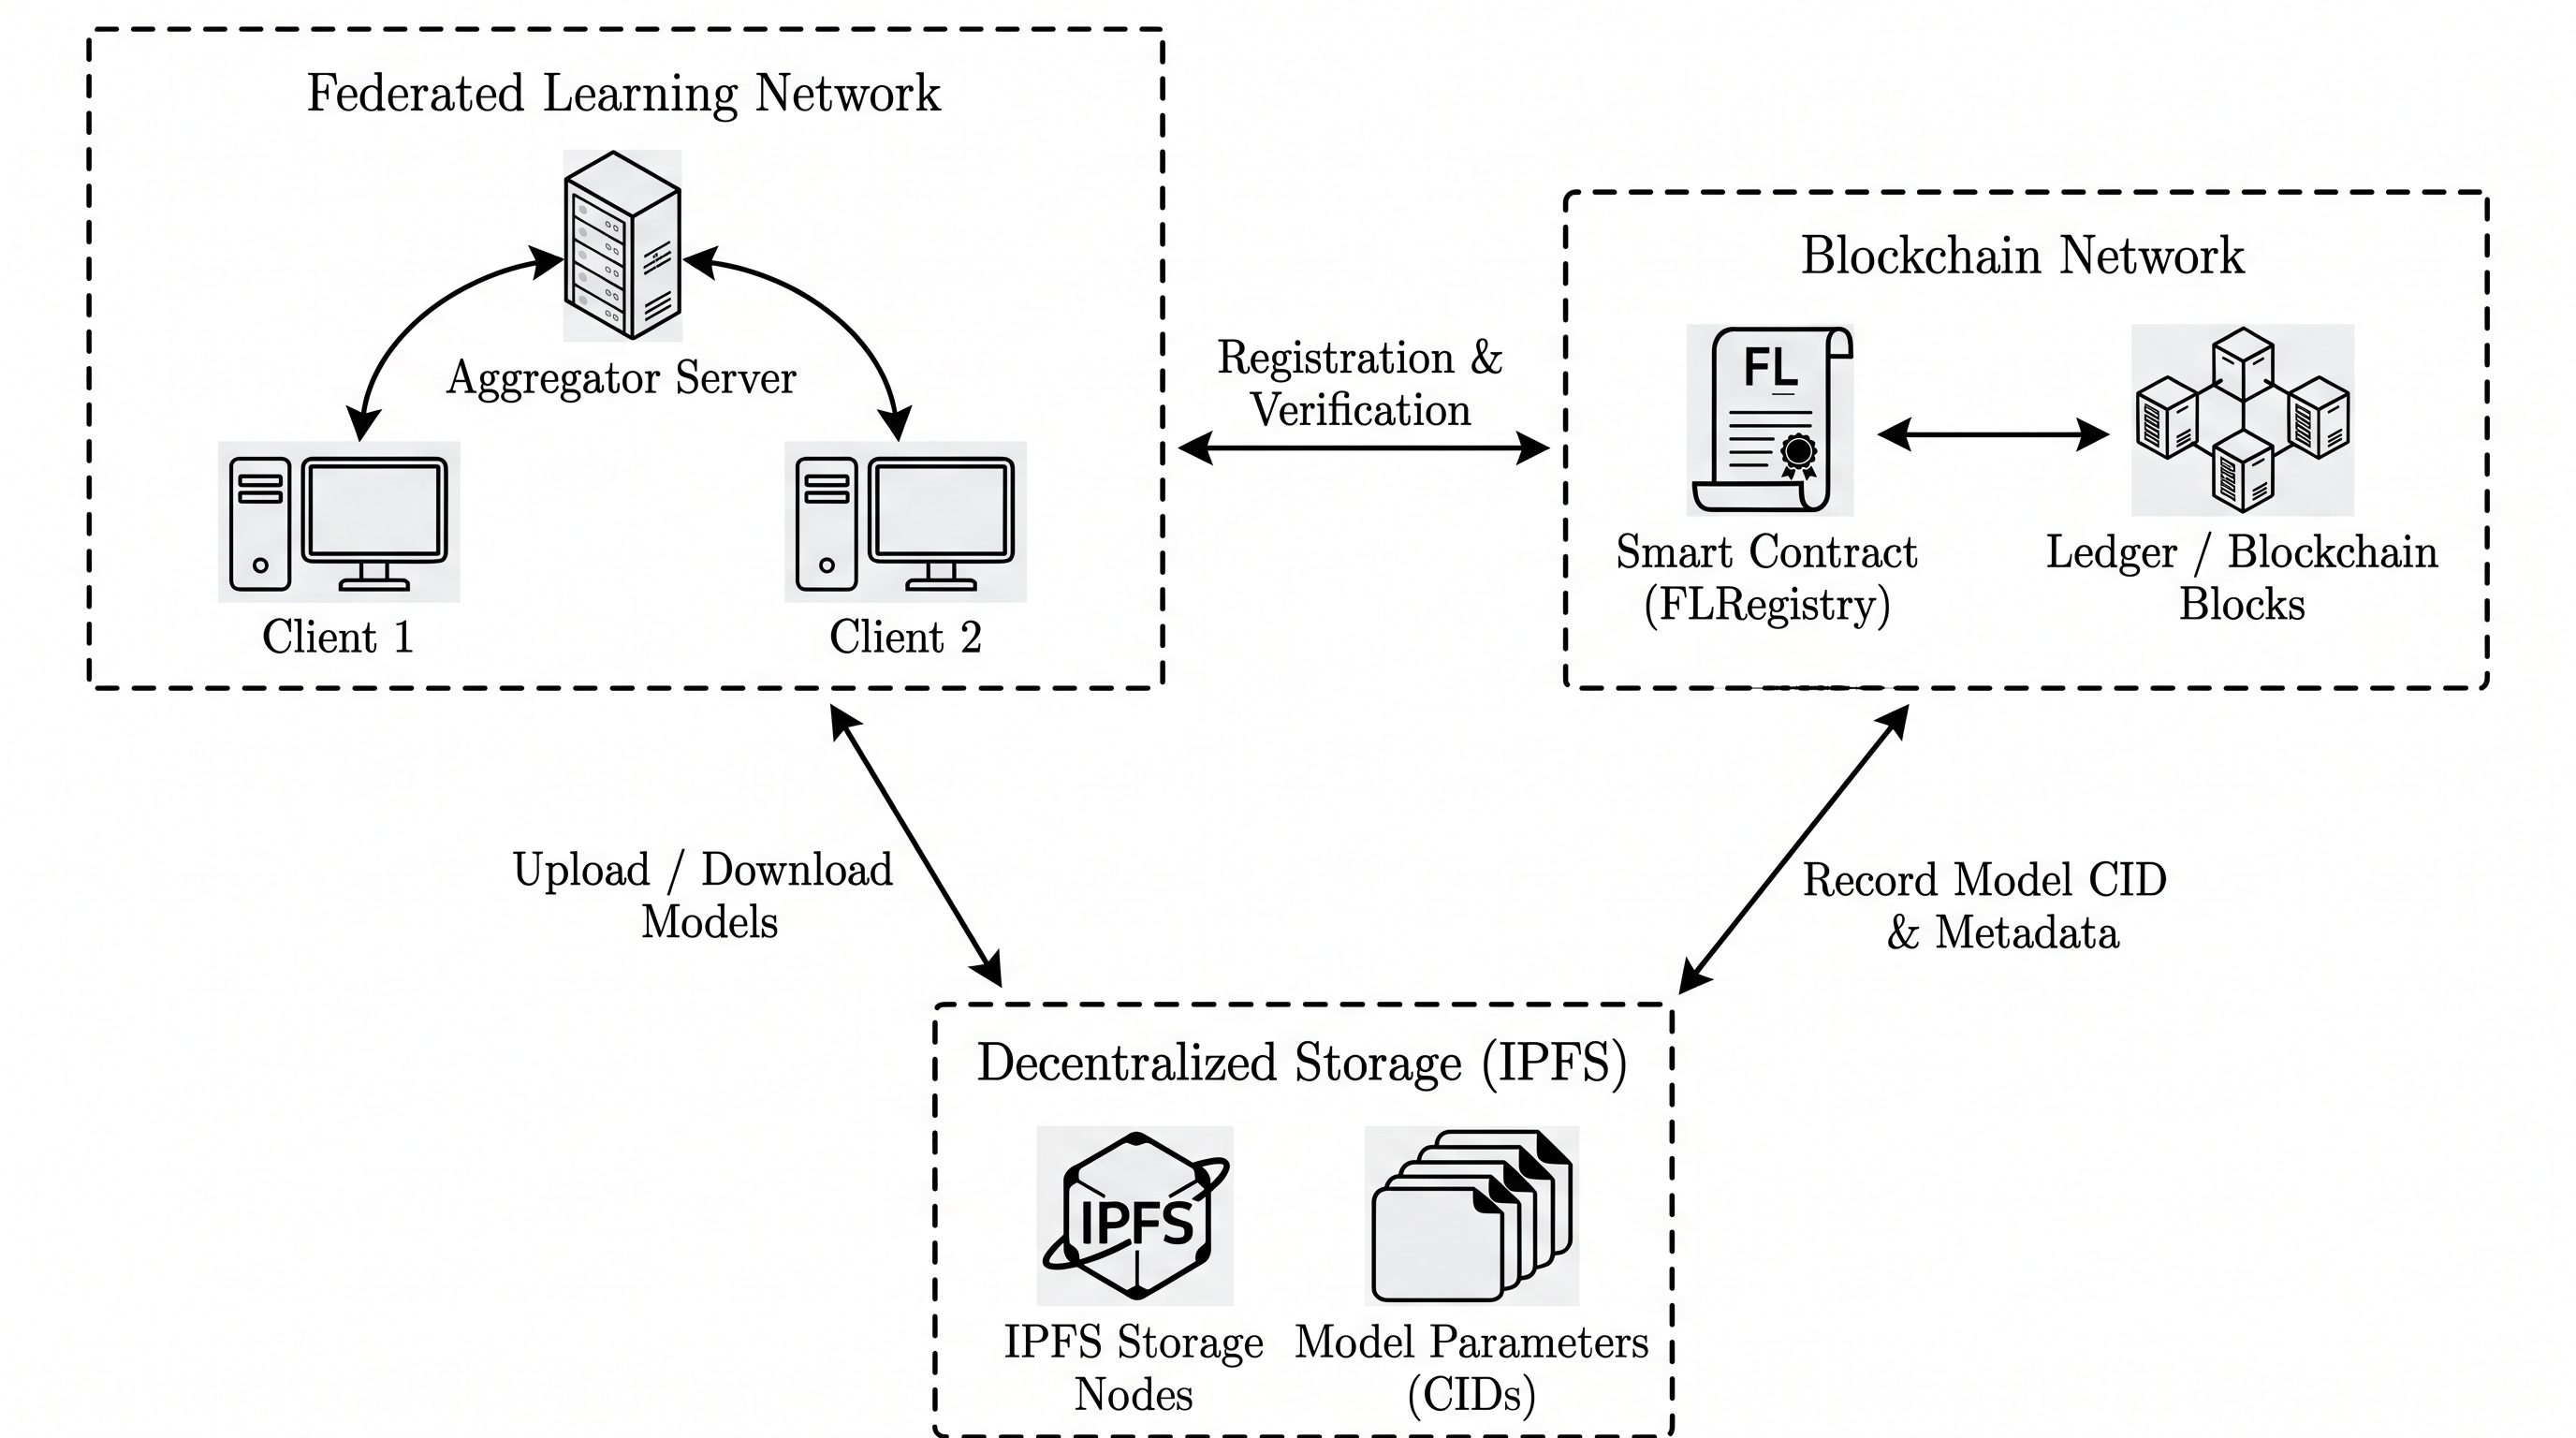
\includegraphics[width=0.88\textwidth]{figures/ArqSistema.png}
    \caption{Overall hybrid system architecture: decoupling between federated computation (Flower), off-chain parameter storage (IPFS), and immutable traceability logging (Hyperledger Besu with IBFT 2.0).}
    \label{fig:arq_sistema}
\end{figure}

\subsection{Smart Contract Design: FLRegistry}
Governance and audit logic are encapsulated within the \texttt{FLRegistry} smart contract, implemented in Solidity (compiler version \texttt{0.8.10}). Its primary objective is to maintain a deterministic, chronological audit log of each federated round without storing massive numerical parameter matrices on-chain.

\subsubsection{Data Structures and Persistence}
The core entity within the contract is the \texttt{ModelRound} structure, defined as:
\begin{verbatim}
struct ModelRound {
    uint256 roundNum;
    string modelHash;
    address author;
    uint256 timestamp;
}
\end{verbatim}
where \texttt{roundNum} indexes the federated iteration, \texttt{modelHash} stores the IPFS Content Identifier (CIDv0, encapsulating the SHA-256 multihash of the serialized model), \texttt{author} records the Ethereum public address of the sender (\texttt{msg.sender}), and \texttt{timestamp} captures the block validation timestamp.

Contract state is organized through two complementary mappings:
\begin{itemize}
    \item \texttt{mapping(uint256 => ModelRound) public history}: sequentially records the global models aggregated by the coordinator at the conclusion of each round $t$.
    \item \texttt{mapping(uint256 => mapping(address => ModelRound)) public clientHistory}: indexes the individual local contributions submitted by each client in each round, enabling granular forensic auditing.
\end{itemize}

Additionally, state pointers \texttt{latestRound} and boolean flag \texttt{hasModel} are maintained to facilitate direct and constant-time read access without requiring iterative storage scans.

\subsubsection{State-Modifying Primitives and Access Control}
The contract exposes two state-modifying transactional functions that emit the decoupled \texttt{ModelUpdated} event:
\begin{itemize}
    \item \texttt{registerClientModel(uint256 round, string memory hash)}: Invoked by each edge client $k$ upon completing local training, immutably binding the CID of its contribution to its Ethereum address (\texttt{msg.sender}).
    \item \texttt{updateModel(uint256 round, string memory hash)}: Invoked operationally by the aggregation coordinator after executing the aggregation algorithm. To enforce consortium governance and prevent unauthorized participants or rogue nodes from submitting fraudulent global models, this function is guarded by the \texttt{onlyServer} access control modifier:
    \begin{verbatim}
modifier onlyServer() {
    require(msg.sender == serverAddress, 
            "Unauthorized sender");
    _;
}
    \end{verbatim}
    where \texttt{serverAddress} is initialized in the contract constructor with the authorized coordinator public address (which can be reassigned or governed via consortium multi-signature schemes). Consequently, the EVM deterministically reverts any unauthorized call to \texttt{updateModel}.
\end{itemize}

\subsubsection{Read and Verification Primitives}
To avoid imposing execution costs during routine checks, model verification queries are implemented as \texttt{view} functions, resolved locally at the JSON-RPC node without consuming gas:
\begin{itemize}
    \item \texttt{getLastModel()}: Enables any client to retrieve the CID of the latest consolidated global model along with its validation timestamp.
    \item \texttt{getClientModel(uint256 round, address client)}: Enables the coordinator and external auditors to cross-check the CID reported by a client against its signed on-chain record.
\end{itemize}

\subsubsection{Model-Agnostic Design and Generalization}
The proposed framework is architecturally and operationally agnostic to neural network topology, data modality, and training framework. Because \texttt{FLRegistry} processes exclusively uniform 46-character string identifiers (the IPFS CIDs encapsulating the multihash digest of the serialized weights), EVM gas costs remain predictable and entirely decoupled from model parameter dimensions—whether the weights represent a shallow classifier, a deep convolutional network, or a Transformer architecture. Similarly, the IPFS storage plane treats serialized parameters as generic byte payloads, making this bidirectional verification protocol directly applicable across diverse modalities (tabular data, time series, acoustic signals, or computer vision) and federated optimization algorithms.

\subsection{Operational Workflow and Bidirectional Cross-Verification}
The federated lifecycle consists of a one-time bootstrap phase followed by an iterative protocol featuring strict bidirectional verification, detailed below:

\subsubsection{Phase 0: Bootstrap and Baseline Model (Round 0)}
Prior to concurrent training execution:
\begin{enumerate}
    \item The Hyperledger Besu network operating under IBFT 2.0 consensus and the IPFS daemon are initialized.
    \item \texttt{FLRegistry} is deployed, and its contract address and ABI are published in a shared configuration manifest.
    \item The coordinator instantiates the initial model parameters $w^{(0)}$, serializes them, and uploads them to IPFS, obtaining the initial identifier $\text{CID}_0$.
    \item The coordinator executes \texttt{updateModel(0, }$\text{CID}_0$\texttt{)}, establishing an auditable cryptographic baseline for all participants.
\end{enumerate}

\subsubsection{Phase 1: Downward Verification (Client Verifies Server)}
Upon receiving the round start signal and candidate weights $w_{cand}^{(t)}$ via gRPC (Figure~\ref{fig:flujo_cliente_verif}):
\begin{enumerate}
    \item The client queries the blockchain by calling \texttt{getLastModel()}, retrieving the officially committed $\text{CID}_{reg}^{(t-1)}$.
    \item The client fetches the referenced model artifact from IPFS and performs an exhaustive, element-wise numerical comparison across all tensor layers against $w_{cand}^{(t)}$ (verifying parametric equality within a floating-point tolerance of $\epsilon = 10^{-7}$).
    \item If any discrepancy is detected between the delivered weights and the on-chain commitment, the client \textbf{aborts training immediately}, effectively neutralizing split-view attacks where a compromised coordinator attempts to distribute biased models selectively to specific clients.
\end{enumerate}

\begin{figure}[htbp]
    \centering
    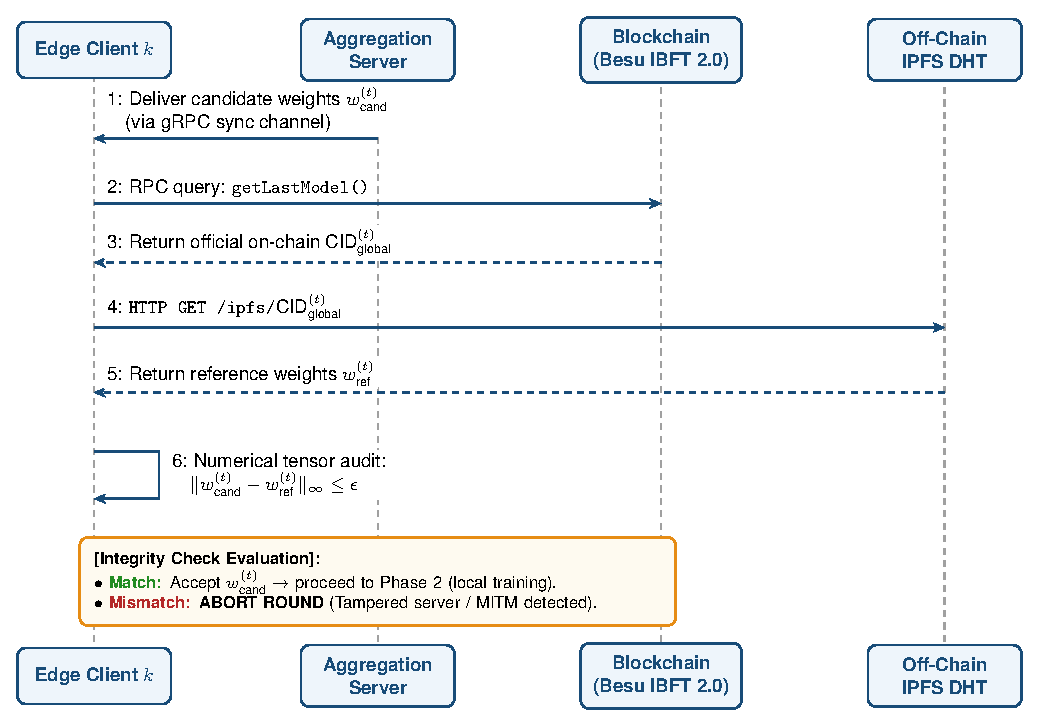
\includegraphics[width=\columnwidth]{figures/flujo_fase1_verificacion_descendente.pdf}
    \caption{Phase 1: Downward verification at the edge client: validating received candidate weights against the on-chain registered CID retrieved from IPFS.}
    \label{fig:flujo_cliente_verif}
\end{figure}

\subsubsection{Phase 2: Local Training and Contribution Commitment}
If the downward verification check passes successfully (Figure~\ref{fig:flujo_cliente_entreno}):
\begin{enumerate}
    \item The client performs local training on its private data partition.
    \item It serializes the updated local weight vector $w_k^{(t)}$ and uploads it to IPFS, obtaining $\text{CID}_k^{(t)}$.
    \item It broadcasts a signed transaction calling \texttt{registerClientModel(}$t$, $\text{CID}_k^{(t)}$\texttt{)} and awaits confirmation within an IBFT 2.0 block receipt.
    \item It returns the parameter payload along with $\text{CID}_k^{(t)}$ and its public key to the Flower coordinator.
\end{enumerate}

\begin{figure}[htbp]
    \centering
    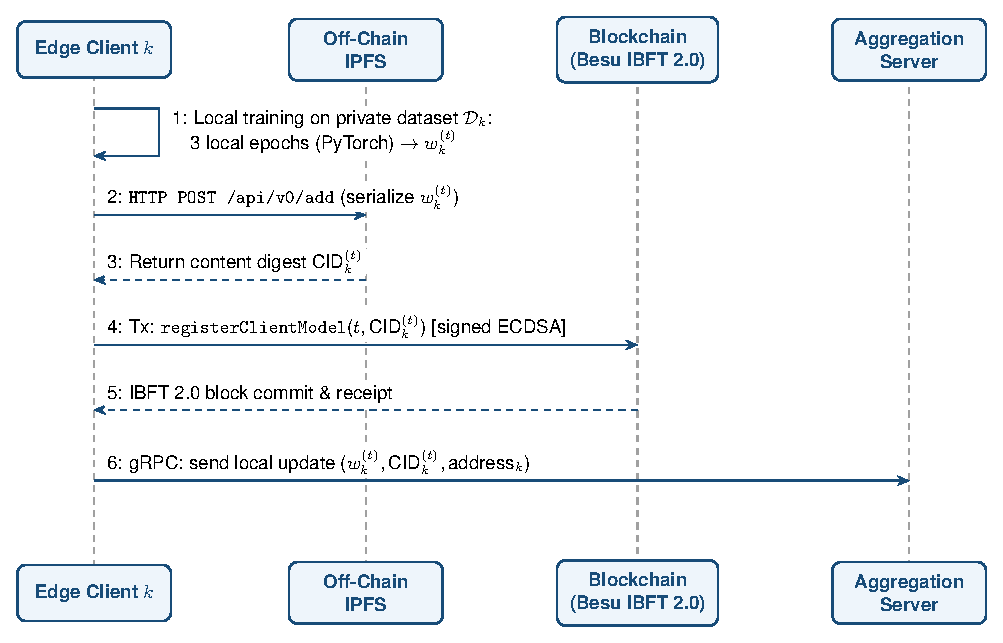
\includegraphics[width=\columnwidth]{figures/flujo_fase2_entrenamiento_registro.pdf}
    \caption{Phase 2: Local training at the client, parameter upload to IPFS, and signed transaction commitment to Hyperledger Besu.}
    \label{fig:flujo_cliente_entreno}
\end{figure}

\subsubsection{Phase 3: Upward Verification and Global Aggregation}
Upon receiving client updates at the aggregation coordinator (Figure~\ref{fig:flujo_servidor_agregacion}):
\begin{enumerate}
    \item For each client $k$, the server receives parameter payload $w_k^{(t)}$, identifier $\text{CID}_{k,\text{gRPC}}^{(t)}$, and client address $\text{address}_k$.
    \item \textbf{In-memory integrity verification:} The server deterministically computes the cryptographic digest of the received weight vector: $\text{CID}_{k,\text{calc}}^{(t)} = \text{Hash}(w_k^{(t)})$.
    \item \textbf{On-chain verification and double cross-check:} The server queries \texttt{getClientModel($t$, address$_k$)} from \texttt{FLRegistry}, retrieving $\text{CID}_{k,\text{onchain}}^{(t)}$, and enforces strict double equality:
    \begin{equation}
    \text{CID}_{k,\text{calc}}^{(t)} == \text{CID}_{k,\text{gRPC}}^{(t)} == \text{CID}_{k,\text{onchain}}^{(t)}
    \end{equation}
    This dual check counters two complementary threat vectors: if a malicious client commits a valid CID on Besu but transmits tampered weights over gRPC, or if a network adversary alters parameters in transit, $\text{CID}_{k,\text{calc}}^{(t)} \neq \text{CID}_{k,\text{onchain}}^{(t)}$; similarly, if the gRPC-reported CID does not match the signed transaction on Besu, verification fails immediately. In either case, the contribution is discarded prior to aggregation.
    \item The server executes FedAvg aggregation exclusively over verified contributions:
    \begin{equation}
    w^{(t+1)} = \sum_{k \in \mathcal{K}_{valid}} \frac{n_k}{n_{valid}} \, w_k^{(t)}
    \end{equation}
    where $n_k$ is the local sample count of client $k$ and $n_{valid} = \sum_{k \in \mathcal{K}_{valid}} n_k$.
    \item The server uploads the aggregated model to IPFS, obtaining $\text{CID}_{global}^{(t+1)}$, and anchors it on Besu by executing \texttt{updateModel(}$t+1$, $\text{CID}_{global}^{(t+1)}$\texttt{)}. Because \texttt{updateModel} is restricted by \texttt{onlyServer}, no outside party can overwrite the consolidated global model.
\end{enumerate}

\begin{figure}[htbp]
    \centering
    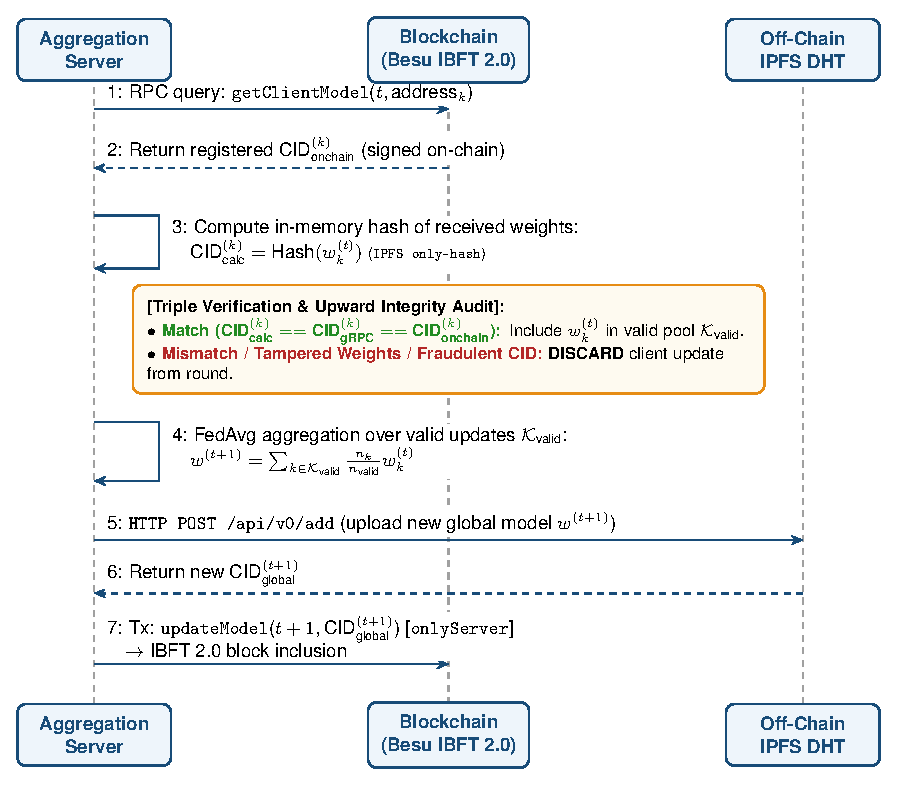
\includegraphics[width=\columnwidth]{figures/flujo_fase3_verificacion_agregacion.pdf}
    \caption{Phase 3: Upward verification at the aggregation coordinator: tensor integrity validation, on-chain cross-check, FedAvg aggregation, and global round commitment.}
    \label{fig:flujo_servidor_agregacion}
\end{figure}

\subsection{Ex-Post Auditing and Verifiability of FedAvg}
\label{subsec:auditoria_fedavg}
A distinctive architectural capability enabled by our hybrid decoupling is the ability to deterministically verify coordinator honesty retrospectively (\textit{ex-post}). In conventional federated setups, the aggregation server operates as a trusted black box: participants must trust that aggregated weights $w^{(t+1)}$ faithfully represent a weighted average over received contributions, without arbitrary omissions, unauthorized weight injections, or stealthy backdoors.

In our decoupled architecture, every round $t$ produces an immutable and reproducible audit trail linking the blockchain ledger to the content repository:
\begin{enumerate}
    \item \textbf{Participant identification $\mathcal{K}_t$:} Because Solidity \texttt{mapping} structures are non-iterable by EVM design, active participants in round $t$ are discovered deterministically by querying \texttt{ModelUpdated(round, modelHash, author)} event logs emitted during \texttt{registerClientModel} calls via standard RPC methods (\texttt{eth\_getLogs}), or from the permissioned consortium whitelist.
    \item \textbf{Local weight commitments:} Each participating client $k \in \mathcal{K}_t$ signs and registers its $\text{CID}_k^{(t)}$ in \texttt{clientHistory}, accessible via \texttt{getClientModel($t$, address$_k$)}.
    \item \textbf{Sample weighting factors $n_k$:} In balanced, homogeneous deployments (such as the evaluated experimental benchmark, where clients operate over equivalent IID partitions, $n_k = N / |\mathcal{K}_t|$), weighting factors are symmetric ($n_k / \sum n_j = 1/|\mathcal{K}_t|$). In heterogeneous settings (non-IID), scalar values $n_k$ can be embedded within the IPFS metadata descriptor or included as an event parameter, allowing exact reconstruction without exposing raw training samples.
    \item \textbf{Global model commitment:} The coordinator seals $\text{CID}_{\text{global}}^{(t+1)}$ in \texttt{history}, accessible via \texttt{getLastModel()} or direct round indexing.
\end{enumerate}

From this immutable audit trail, any consortium member or independent third-party auditor can execute a deterministic aggregation check without accessing private datasets:
\begin{enumerate}
    \item \textbf{Artifact retrieval:} The auditor queries Besu to retrieve active clients $\mathcal{K}_t$ and their committed $\text{CID}_k^{(t)}$, then downloads the binary parameter tensors $w_k^{(t)}$ from IPFS.
    \item \textbf{Input integrity validation:} It verifies that for each client $k \in \mathcal{K}_t$, the cryptographic digest of the downloaded weights strictly matches the on-chain committed $\text{CID}_k^{(t)}$.
    \item \textbf{Mathematical aggregation reconstruction:} It computes the canonical FedAvg aggregation:
    \begin{equation}
    \hat{w}^{(t+1)} = \sum_{k \in \mathcal{K}_t} \frac{n_k}{\sum_{j \in \mathcal{K}_t} n_j} \, w_k^{(t)}
    \end{equation}
    \item \textbf{Global model cross-check:} It serializes $\hat{w}^{(t+1)}$ and computes its content identifier $\text{CID}_{audit}^{(t+1)} = \text{Hash}(\hat{w}^{(t+1)})$. Finally, it evaluates whether $\text{CID}_{audit}^{(t+1)} == \text{CID}_{global}^{(t+1)}$, registered in \texttt{FLRegistry}.
\end{enumerate}
If $\text{CID}_{audit}^{(t+1)} \neq \text{CID}_{global}^{(t+1)}$, any coordinator deviation—whether due to biased weighting, participant omission, or unauthorized parameter tampering—is cryptographically, publicly, and non-repudiably proven. This verifiability transforms the centralized aggregator into a strictly accountable, provably honest orchestrator.

\subsection{Threat Model and Security Scope}
\label{subsec:modelo_amenazas}
To clearly delineate the defensive guarantees provided by the framework, this section defines the threat model, distinguishing between vulnerabilities mitigated by design and those that lie outside our scope.

\subsubsection{Mitigated Threats (In-Scope)}
\begin{itemize}
    \item \textbf{Man-in-the-Middle tampering}: A network adversary intercepting the gRPC channel who attempts to alter local parameter tensors sent to the server or global models delivered to clients. Discrepancies are intercepted immediately through element-wise numerical checks and on-chain CID verification.
    \item \textbf{Server equivocation / split-view attacks}: An untrusted or compromised coordinator attempting to deceive specific edge nodes by distributing divergent or altered global models (e.g., to facilitate active gradient inversion or localized performance degradation, as formalized by Carletti et al.~\cite{carletti2026detectability}). Because clients accept only weights whose content identifier strictly matches the authoritative commitment in \texttt{FLRegistry}, divergent distribution attempts are blocked locally.
    \item \textbf{Unauthorized global model injection}: Attempts by rogue participants or external adversaries to commit unauthorized global models to the blockchain are rejected by the EVM through the \texttt{onlyServer} modifier.
    \item \textbf{Contribution repudiation}: Elliptic curve digital signatures (ECDSA secp256k1) underpinning Hyperledger Besu transactions prevent participants from repudiating submitted parameter updates.
\end{itemize}

\subsubsection{Out-of-Scope Threats and System Boundaries}
\begin{itemize}
    \item \textbf{Semantic data and model poisoning with valid signatures}: If an adversary trains on poisoned datasets (e.g., label flipping or stealthy backdoors) but legitimately signs and registers the resulting model updates on Besu, cryptographic verification confirms provenance and integrity but cannot assess gradient statistical quality. Defense against semantic attacks requires pairing on-chain traceability with robust Byzantine aggregation rules (e.g., Krum~\cite{blanchard2017byzantine}, Median, Trimmed Mean) or forensic ex-post auditing of flagged contributions.
    \item \textbf{Private key compromise}: Cryptographic guarantees assume secure client key management. In industrial deployments, private keys must be secured via Hardware Security Modules (HSMs) or Trusted Execution Environments (TEEs).
    \item \textbf{Inference and gradient inversion attacks}: While our framework ensures integrity and provenance, it does not incorporate Differential Privacy (DP) or Secure Multiparty Computation (SMPC) to obfuscate shared gradients against reconstruction attacks~\cite{carletti2026detectability}.
\end{itemize}

\subsubsection{Privacy and Weight Exposure on IPFS}
On a public IPFS instance, any node knowing a model CID could retrieve parameter tensors and potentially attempt training data extraction. To protect model privacy in consortium deployments with stringent confidentiality requirements (e.g., autonomous fleets or healthcare), the framework supports two hardening mechanisms:
\begin{enumerate}
    \item \textbf{Private IPFS Swarm}: Configuring the IPFS daemon in private swarm mode using a shared key (\texttt{swarm.key}) and setting \texttt{LIBP2P\_FORCE\_PNET=1}. This prevents unauthorized nodes from connecting to the P2P overlay or fetching storage blocks.
    \item \textbf{Payload encryption at rest}: Encrypting serialized parameter vectors (e.g., using AES-256-GCM) prior to IPFS publication. Symmetric decryption keys can be distributed via asymmetric public-key cryptography to authorized consortium members or managed through Attribute-Based Encryption (ABE).
\end{enumerate}

% !TeX root = ../main.tex
\section{Implementación y Entorno Experimental}
\label{sec:implementacion}

Con el fin de aislar y evaluar cuantitativamente el sobrecoste introducido por la capa de trazabilidad y auditoría, se desplegó un banco de pruebas experimental representativo de un entorno de computación distribuida vehicular.

\subsection{Infraestructura de Hardware y Software}
La evaluación empírica se llevó a cabo utilizando dos estaciones físicas interconectadas en la misma red de área local (LAN), cuyas especificaciones técnicas se detallan en la Tabla~\ref{tab:testbed_hardware}:
\begin{itemize}
    \item \textbf{Estación 1 (Servidor, Validadores e IPFS)}: Aloja el servidor agregador Flower, el daemon IPFS y la totalidad de los nodos validadores de la red permisionada Hyperledger Besu (los 4 validadores en las configuraciones E1 y E4, y los 7 validadores en E5). Cada validador se ejecuta de forma contenerizada como un servicio independiente mediante Docker Compose, interconectados a través de una red virtual en puente (\textit{bridge}) que emula el mallado de consenso del consorcio vehicular y expone el puerto JSON-RPC del nodo validador principal como pasarela para el resto de entidades.
    \item \textbf{Estación 2 (Nodos de Borde / Clientes)}: Aloja y ejecuta los clientes de entrenamiento federado (\textit{members} 2 y 3), los cuales se comunican con el servidor y la red blockchain a través de la conexión LAN.
\end{itemize}

\begin{table}[htbp]
\caption{Especificaciones del banco de pruebas experimental.}\label{tab:testbed_hardware}
\begin{tabular*}{\textwidth}{@{\extracolsep\fill}lll}
\toprule
\textbf{Parámetro} & \textbf{Estación 1 (Servidor/RPC)} & \textbf{Estación 2 (Clientes)} \\
\midrule
Procesador & Intel Core i5-1135G7 & Intel Core i7-9700 \\
Frecuencia base & 2,40 GHz & 3,00 GHz \\
Núcleos / Hilos & 4 núcleos / 8 hilos & 8 núcleos / 8 hilos \\
Memoria RAM & 7,6 GB (asignada en WSL2) & 8,0 GB \\
Sistema Operativo & Ubuntu 22.04 LTS (WSL2) & Windows 11 \\
\bottomrule
\end{tabular*}
\end{table}

El stack de software está compuesto por Hyperledger Besu operando con el algoritmo de consenso QBFT / IBFT 2.0 y un periodo de emisión de bloques fijado en 5 segundos (\texttt{blockperiodseconds: 5}), con soporte de transacciones privadas mediante Tessera y orquestación con Docker Compose; el daemon IPFS Kubo (\texttt{v0.32.1}); Python \texttt{3.12} con PyTorch~\cite{paszke2019pytorch} para la inferencia y optimización neuronal; Flower (\texttt{flwr})~\cite{beutel2020flower} para la coordinación gRPC de la federación; y la biblioteca \texttt{web3.py} para la conectividad JSON-RPC con la EVM. Todos los contratos inteligentes, configuraciones de red y scripts de orquestación se encuentran disponibles en el repositorio público~\url{https://github.com/dpz6-ua/Blockchain_ML}.

Las dos estaciones se encuentran comunicadas a través de un enlace de red de área local inalámbrico (Wi-Fi 802.11ac a 5~GHz), registrando una latencia media de ida y vuelta (\textit{RTT ping}) de $3{,}8 \pm 1{,}1$~ms y un ancho de banda sostenido de 100~Mbps. El tamaño del modelo neuronal serializado (\texttt{NetCliente}) es de exactamente $1{,}95$~MB en formato binario. Para favorecer un rendimiento ágil en la capa de almacenamiento distribuido durante el ciclo federado, la subida a IPFS se efectúa mediante la API HTTP en el endpoint \texttt{/api/v0/add?pin=false}, lo que permite generar el identificador CID e incorporar el bloque al repositorio local en milisegundos sin la sobrecarga síncrona del anclaje. Conviene puntualizar que, si bien la directiva \texttt{pin=false} optimiza la latencia inmediata entre rondas, no garantiza por sí misma la disponibilidad o persistencia indefinida de los artefactos frente a futuros procesos de recolección de basura (\textit{garbage collection}) del daemon IPFS, requiriendo en despliegues productivos políticas de anclaje explícito o sincronización en un clúster IPFS persistente.

\subsection{Modelo Neuronal y Conjunto de Datos Vehicular}
Como caso de uso para simular un sistema de asistencia a la conducción en vehículos conectados y autónomos (CAV)~\cite{chellapandi2024federated}, se adoptó el dataset de clasificación de eventos de tráfico del grupo CloudLab-AIA~\cite{cloudlabaia_flblockchain}. 

El problema consiste en una tarea de clasificación multiclase orientada a la detección en carretera con cuatro categorías:
\begin{enumerate}
    \item Accidente vial (\texttt{accident}).
    \item Congestión o tráfico denso (\texttt{dense\_traffic}).
    \item Condiciones meteorológicas adversas (\texttt{meteorology}).
    \item Flujo de tráfico fluido (\texttt{sparse\_traffic}).
\end{enumerate}

El conjunto de datos comprende un total de 3.415 imágenes distribuidas en: meteorología adversa (1.027), tráfico fluido (947), tráfico denso (778) y accidentes (663). Las imágenes se preprocesan mediante reescalado a una resolución de $32 \times 32$ píxeles en tres canales cromáticos (RGB) y normalización estándar. Para preservar la comparabilidad estadística y eliminar sesgos de distribución, el conjunto de datos se reparte entre los $K=2$ clientes según un esquema independiente e idénticamente distribuido (IID).

El modelo implementado (\texttt{NetCliente}) es una red neuronal convolucional (CNN) estructurada en dos bloques convolucionales consecutivos (con kernels de $3 \times 3$, función de activación ReLU y submuestreo por \textit{Max Pooling}), seguidos de dos capas densas completamente conectadas (\textit{fully connected}) que proyectan el vector de características hacia las 4 neuronas de salida. El entrenamiento se realiza mediante la función de pérdida de entropía cruzada (\textit{Cross-Entropy Loss}) y el algoritmo de optimización Adam con una tasa de aprendizaje $\eta = 10^{-3}$, configurando un tamaño de lote (\textit{batch size}) de 16 muestras en entrenamiento y 32 en evaluación, 3 épocas locales de entrenamiento por ronda y un horizonte total de 30 rondas federadas.

Es importante remarcar que el propósito primordial de este estudio no radica en diseñar un modelo convolucional óptimo ni en maximizar su precisión de clasificación, sino en utilizar la arquitectura de aprendizaje federado como un banco de pruebas realista para generar y analizar métricas cuantitativas del sistema (sobrecoste temporal, escalabilidad y consumo de gas). La optimización del modelo (ajuste de hiperparámetros, mitigación del sobreajuste o empleo de arquitecturas más profundas) se plantea deliberadamente como trabajo futuro, actuando aquí la red neuronal como una carga de trabajo experimental representativa. De este modo, la arquitectura desacoplada resulta potencialmente aplicable a otros dominios de aprendizaje distribuido (tales como la monitorización médica, redes inteligentes o finanzas colaborativas), donde la lógica de auditoría en la Blockchain permanece análoga y únicamente el tiempo de transferencia y cálculo de hash off-chain en IPFS escala con el volumen de parámetros del modelo serializado.

\subsection{Matriz de Configuraciones Experimentales}
Para desglosar y desacoplar de forma analítica el impacto individual de cada componente, se diseñaron cinco configuraciones experimentales (E1 a E5), resumidas en la Tabla~\ref{tab:configuraciones}.

\begin{table}[htbp]
\caption{Matriz de configuraciones experimentales evaluadas.}\label{tab:configuraciones}
\begin{tabular*}{\textwidth}{@{\extracolsep\fill}ccccc}
\toprule
\textbf{ID Exp.} & \textbf{Estaciones} & \textbf{Capa Blockchain} & \textbf{Validadores} & \textbf{Objetivo} \\
\midrule
E1 & 1 & Sí & 4 & Sobrecarga BC local \\
E2 & 1 & No & --- & Baseline local \\
E3 & 2 & No & --- & Baseline distribuido \\
E4 & 2 & Sí & 4 & Sobrecarga BC distribuida \\
E5 & 2 & Sí & 7 & Escalabilidad IBFT 2.0 \\
\bottomrule
\end{tabular*}
\end{table}

Este diseño metodológico permite efectuar comparaciones controladas de una sola variable:
\begin{itemize}
    \item \textbf{Coste directo de Blockchain}: Comparación de E1 vs. E2 en entorno monomáquina, y de E4 vs. E3 en entorno distribuido en red.
    \item \textbf{Efecto de la distribución física}: Comparación de E2 vs. E3 (sin Blockchain) y de E1 vs. E4 (con Blockchain de 4 validadores).
    \item \textbf{Escalado del consenso BFT}: Comparación de E4 (4 validadores) vs. E5 (7 validadores), evaluando la penalización de latencia al elevar la tolerancia a fallos de $f=1$ a $f=2$.
\end{itemize}


% !TeX root = ../main.tex
\section{Experimental Evaluation and Results}
\label{sec:evaluacion}

This section quantitatively analyzes the performance of the proposed architecture across the experimental testbed, directly addressing the core research questions: the temporal overhead of the auditability layer, the impact of physical resource decoupling, the latency impact of expanding the IBFT 2.0 validator committee, the empirical resilience against adversarial tampering attacks, and the predictability of EVM gas consumption. To ensure statistical soundness and experimental reproducibility, each of the five experimental configurations ($E_1$ to $E_5$) was evaluated across 3 complete, independent executions of 30 federated rounds each, yielding a corpus of 15 executions and 450 total federated rounds ($N_{\text{total}} = 450$). We note that the model convergence trajectory is identical with or without the blockchain layer, as the traceability framework operates fully decoupled and does not modify training tensors or gradients.

\subsection{Mathematical Formalization of Performance Metrics}
To isolate the latency imposed by each system component, the total round time at the edge nodes ($T_{\text{client}}$) and at the central coordinator ($T_{\text{server}}$) during iteration $t$ is analytically defined as:
\begin{align}
T_{\text{client}}^{(t)} &= t_{\text{verif\_desc}}^{(t)} + t_{\text{train}}^{(t)} + t_{\text{ipfs\_up}}^{(t)} + t_{\text{tx\_besu}}^{(t)} \label{eq:t_client} \\
T_{\text{server}}^{(t)} &= t_{\text{wait}}^{(t)} + t_{\text{verif\_asc}}^{(t)} + t_{\text{fedavg}}^{(t)} \nonumber \\
&\quad + t_{\text{ipfs\_global}}^{(t)} + t_{\text{block\_confirm}}^{(t)} \label{eq:t_server}
\end{align}
where $t_{\text{verif\_desc}}$ denotes local downward verification against the Besu CID; $t_{\text{train}}$, gradient computation time in PyTorch; $t_{\text{ipfs\_up}}$, binary model publication to IPFS; $t_{\text{tx\_besu}}$, transaction issuance and confirmation for \texttt{registerClientModel}; $t_{\text{wait}}$, the coordinator gRPC reception window; $t_{\text{verif\_asc}}$, on-chain validation via \texttt{getClientModel}; $t_{\text{fedavg}}$, matrix aggregation; and $t_{\text{block\_confirm}}$, IBFT 2.0 block confirmation following \texttt{updateModel}.

These two timing perspectives provide complementary system insights:
\begin{itemize}
    \item \textbf{Client cycle time ($T_{\text{client}}$, reported in Table~\ref{tab:tiempos_resumen}):} Quantifies local computation and communication duration at edge nodes (vehicles), from the receipt of the global model to the confirmation of their contribution on the blockchain. This metric governs client operational autonomy and maintains comparability with prior benchmarks~\cite{cloudlabaia_flblockchain}.
    \item \textbf{End-to-end round time at the server ($T_{\text{server}}$, broken down in Table~\ref{tab:desglose_fases}):} Encompasses the entire round orchestrated by the central coordinator, including gRPC client synchronization and block inclusion of the aggregated global model via \texttt{updateModel} ($\approx 2.8\text{--}5.1$~s additional latency per round).
\end{itemize}

Relative temporal overhead ($\Delta_{\text{overhead}}$) between a secure configuration $E_{\text{BC}}$ and its corresponding baseline $E_{\text{base}}$ is calculated using the distribution medians:
\begin{equation}
\Delta_{\text{overhead}} = \frac{\text{Med}(T_{E_{\text{BC}}}) - \text{Med}(T_{E_{\text{base}}})}{\text{Med}(T_{E_{\text{base}}})} \times 100 \quad [\%] \label{eq:overhead}
\end{equation}

Regarding statistical methodology, the experimental protocol treats the \textbf{15 complete executions} as independent sample units ($N_{\text{runs}} = 3$ independent repetitions per configuration). The 30 consecutive rounds of each run are not treated as independent and identically distributed (i.i.d.) observations, because round $t+1$ depends intrinsically on the model state and system conditions at round $t$. Consequently, all 450 rounds (90 per configuration) are utilized for longitudinal descriptive analysis and trajectory visualization (Figure~\ref{fig:tiempo_todas}), while inter-run reproducibility is quantified via the Standard Error ($SE$) across execution means ($SE = \sigma_{\text{runs}} / \sqrt{N_{\text{runs}}}$).

\subsection{Consolidated Temporal Performance Overview}
Table~\ref{tab:tiempos_resumen} summarizes the per-round client cycle time ($T_{\text{client}}$) across the 15 independent runs (3 per configuration, totaling 90 rounds per environment), reporting the median, mean, inter-run standard deviation ($\sigma_{\text{runs}}$), and standard error ($SE = \sigma_{\text{runs}} / \sqrt{3}$). Figure~\ref{fig:tiempo_todas} depicts the continuous time-series trajectories across all rounds.

\begin{table}[htbp]
\caption{Consolidated per-round client cycle time ($T_{\text{client}}$) across 15 independent executions (3 per configuration, 30 rounds/run). Values of $\sigma_{\text{runs}}$ and $SE$ quantify dispersion and standard error across the 3 independent execution means ($SE = \sigma_{\text{runs}} / \sqrt{3}$).}\label{tab:tiempos_resumen}
\small
\setlength{\tabcolsep}{3pt}
\begin{tabular*}{\textwidth}{@{\extracolsep\fill}cccccccc}
\toprule
\textbf{Exp.} & \textbf{Nodes} & \textbf{Configuration} & \textbf{Runs} & \textbf{Median (s)} & \textbf{Mean (s)} & \textbf{$\sigma_{\text{runs}}$ (s)} & \textbf{SE (s)} \\
\midrule
$E_1$ & 1 & 4 val · with BC & 3 & \textbf{85.42} & 97.09 & 20.01 & 11.55 \\
$E_2$ & 1 & Baseline without BC & 3 & \textbf{75.70} & 76.45 & 1.65 & 0.95 \\
\midrule
$E_3$ & 2 & Baseline without BC & 3 & \textbf{66.62} & 67.62 & 2.29 & 1.32 \\
$E_4$ & 2 & 4 val · with BC & 3 & \textbf{72.96} & 73.29 & 1.28 & 0.74 \\
$E_5$ & 2 & 7 val · with BC & 3 & \textbf{73.35} & 74.40 & 0.54 & 0.31 \\
\bottomrule
\end{tabular*}
\end{table}

\begin{figure}[htbp]
    \centering
    \includegraphics[width=\columnwidth]{figuras/tiempo_ronda_todas.png}
    \caption{Comparison of client cycle time ($T_{\text{client}}$) across federated rounds for the five evaluated configurations.}
    \label{fig:tiempo_todas}
\end{figure}

The multi-run analysis reveals significant differences in operational stability across environments. In the local single-workstation configuration $E_1$, inter-run variability across execution means reached $\sigma_{\text{runs}} = 20.01$~s ($SE = 11.55$~s), with an aggregated longitudinal standard deviation across all 90 rounds of $\sigma_{\text{pool}} = 27.64$~s. This pronounced dispersion occurred because, during single-machine execution, local convolutional training competed directly for CPU and memory resources with eight background Docker containers hosting the Besu validator nodes and the IPFS daemon. Conversely, in the distributed deployment ($E_4$ and $E_5$), inter-run variability dropped markedly ($\sigma_{\text{runs}} \in [0.54, 1.28]$~s and $SE \le 0.74$~s; with pooled longitudinal standard deviations constrained to $\sigma_{\text{pool}} \le 3.92$~s), demonstrating excellent operational stability. Consequently, the \textbf{median} is adopted as the primary metric to isolate intrinsic system performance from transient external perturbations.

\subsection{Isolated Temporal Overhead of the Blockchain Layer}
To evaluate the precise temporal cost incurred by tensor serialization, IPFS upload, ECDSA signing, and IBFT 2.0 consensus, we compare corresponding configurations with and without the security layer (Figure~\ref{fig:coste_bc}):
\begin{itemize}
    \item \textbf{Single-Workstation Scenario ($E_1$ vs. $E_2$)}: Median cycle time increases from 75.70~s to 85.42~s, representing an overhead of \textbf{+9.72~s (+12.8\%)}.
    \item \textbf{Distributed Scenario ($E_3$ vs. $E_4$)}: Median cycle time increases from 66.62~s to 72.96~s, corresponding to an overhead of only \textbf{+6.34~s (+9.5\%)}.
\end{itemize}

\begin{figure}[htbp]
    \centering
    \includegraphics[width=\columnwidth]{figuras/coste_blockchain.png}
    \caption{Temporal overhead induced by blockchain integration in single-workstation and distributed deployments.}
    \label{fig:coste_bc}
\end{figure}

This finding is of particular significance for vehicular and edge systems: when offloading client training to dedicated hardware, the latency impact of the auditability layer remains strictly below 10\%. An additional cost of approximately 6 seconds per round represents a practical, viable trade-off in exchange for end-to-end immutability, non-repudiation, and verifiable integrity.

\subsection{Physical Distribution Effect and Phase Breakdown}
Comparing single-workstation and distributed configurations confirms that physical role decoupling significantly improves overall throughput (Figure~\ref{fig:coste_dist}): round latency decreases both in the baseline setup without blockchain (from 75.70~s to 66.62~s, a 12.0\% speedup) and with blockchain (from 85.42~s to 72.96~s, a 14.6\% speedup).

\begin{figure}[htbp]
    \centering
    \includegraphics[width=\columnwidth]{figuras/coste_distribucion.png}
    \caption{Effect of physical node distribution on cycle time: mitigating CPU/memory contention.}
    \label{fig:coste_dist}
\end{figure}

To analyze the underlying factors driving this behavior, Table~\ref{tab:desglose_fases} provides a fine-grained breakdown of average latency across individual phases at both clients (Station 2) and server (Station 1), demonstrating strict correspondence with the aggregate metrics in Table~\ref{tab:tiempos_resumen}.

\begin{table}[htbp]
\caption{Detailed breakdown of average phase latencies for clients ($T_{\text{client}}$) and coordinator ($T_{\text{server}}$) (in seconds).}\label{tab:desglose_fases}
\begin{tabular*}{\textwidth}{@{\extracolsep\fill}lcccc|cccc}
\toprule
& \multicolumn{4}{c|}{\textbf{Client Phases (Station 2)}} & \multicolumn{4}{c}{\textbf{Server Phases (Station 1)}} \\
\cmidrule(lr){2-5} \cmidrule(lr){6-9}
\textbf{Exp.} & \textbf{Train} & \textbf{Verif.} & \textbf{IPFS} & \textbf{Tx Besu} & \textbf{Wait} & \textbf{Verif.} & \textbf{FedAvg} & \textbf{Block} \\
\midrule
$E_1$ & 94.08 & 0.08 & 0.06 & 2.85 & 98.16 & 0.05 & 0.0065 & 5.14 \\
$E_2$ & 76.45 & 0.00 & 0.00 & 0.00 & 77.02 & 0.00 & 0.0040 & 0.00 \\
\midrule
$E_3$ & 67.62 & 0.00 & 0.00 & 0.00 & 71.07 & 0.00 & 0.0036 & 0.00 \\
$E_4$ & 66.22 & 1.68 & 2.43 & 2.84 & 79.54 & 0.06 & 0.0047 & 2.89 \\
$E_5$ & 65.40 & 1.91 & 3.93 & 2.94 & 82.63 & 0.06 & 0.0079 & 2.99 \\
\bottomrule
\end{tabular*}
\end{table}

The empirical breakdown in Table~\ref{tab:desglose_fases} substantiates three fundamental principles:
\begin{enumerate}
    \item \textbf{Computation decoupling:} In distributed configurations ($E_3$, $E_4$, $E_5$), time dedicated exclusively to PyTorch backpropagation remains constant ($\sim 65.4\text{--}67.6$~s), eliminating the CPU contention observed in $E_1$ ($94.08$~s).
    \item \textbf{Bounded network and verification overhead:} Remote JSON-RPC verification ($1.68\text{--}1.91$~s at clients, $\sim 5$~ms at coordinator), IPFS network transfer ($2.43\text{--}3.93$~s), and in-memory multihash calculation at the coordinator ($\sim 52$~ms in final code, $<0.08\%$ of the cycle) introduce minimal overhead, while FedAvg aggregation is practically instantaneous ($< 8$~ms).
    \item \textbf{Consistency between $T_{\text{client}}$ and $T_{\text{server}}$:} The sum of the four client-side local phases (\textit{Train} + \textit{Verif.} + \textit{IPFS} + \textit{Tx Besu}) strictly accounts for the client cycle time in Table~\ref{tab:tiempos_resumen} (e.g., in $E_4$: $66.22 + 1.68 + 2.43 + 2.84 = 73.17$~s, matching the empirical mean of $73.29$~s). Concurrently, server perspective reflects overall round duration ($T_{\text{server}}$), where the coordinator awaits concurrent client completion (\textit{Wait}, $79.54$~s) and commits the aggregated global model on-chain (\textit{Block}, $2.89$~s), totaling an end-to-end latency of $\approx 82.49$~s.
\end{enumerate}

\subsection{Impact of Validator Committee Size in IBFT 2.0 (4 vs. 7 Validators)}
In permissioned consortium deployments, elevating Byzantine fault tolerance requires expanding the validator committee such that $N \ge 3f + 1$, where $N$ is the total validator count and $f$ is the maximum number of tolerated faulty or adversarial nodes:
\begin{itemize}
    \item 4-validator network ($E_4$): tolerates $f=1$ faulty node; signature quorum $2f+1 = 3$.
    \item 7-validator network ($E_5$): tolerates $f=2$ faulty nodes; signature quorum $2f+1 = 5$.
\end{itemize}
Because all validator instances in our testbed execute containerized on the same physical host, this experiment does not aim to measure wide-area network scalability, but rather to isolate and quantify the direct impact of increasing the validator count and signature quorum on local consensus processing and round duration.

Comparing $E_4$ against $E_5$, median cycle time per round exhibits only a slight change, rising from 72.96~s to 73.35~s (+0.39~s), demonstrating that round cadence remains dominated by local model training rather than consensus messaging.

\begin{figure}[htbp]
    \centering
    \includegraphics[width=\columnwidth]{figuras/tiempo_confirmacion.png}
    \caption{Average on-chain transaction confirmation latency by topology and validator count in Hyperledger Besu.}
    \label{fig:tiempo_confirmacion}
\end{figure}

Isolating \textbf{on-chain transaction confirmation latency} (Figure~\ref{fig:tiempo_confirmacion}) reveals the empirical impact of expanding the consensus committee from 4 to 7 validator nodes in the evaluated testbed:
\begin{itemize}
    \item Client transaction (\texttt{registerClientModel}): mean confirmation latency increases from 2.84~s in $E_4$ to 2.94~s in $E_5$ (+0.10~s).
    \item Coordinator transaction (\texttt{updateModel}): mean confirmation latency increases from 2.89~s in $E_4$ to 2.99~s in $E_5$ (+0.10~s).
\end{itemize}
This symmetric 100~ms increase reflects the empirical consensus communication overhead observed when expanding the validator quorum ($f=1 \to 2$). This indicates that elevated Byzantine resilience can be readily accommodated without disrupting training throughput.

\subsection{Adversarial Robustness and Experimental Attack Verification}
\label{subsec:ataques}
To empirically verify that the architecture actively intercepts real-world adversarial vectors rather than merely logging nominal transactions, controlled attack scenarios were executed via the \texttt{test\_verificacion.py} test suite. The evaluation assesses system behavior against the two primary Byzantine threats in untrusted federated environments: coordinator equivocation or split-view attacks (downward flow) and unauthenticated or tampered client updates (upward flow).

\subsubsection{Test 1: Downward Verification (Tampered Server vs. Edge Client)}
\label{subsubsec:ataque_descendente}
In untrusted federated environments, distributing global weights exposes edge clients to two primary risks: in-transit parameter tampering by network intermediaries (\textit{Man-in-the-Middle}) and malicious server equivocation, where a compromised coordinator delivers divergent or deliberately poisoned models to specific participants. Crucially, the validity of the on-chain global model is strictly governed by the \texttt{onlyServer} access modifier in \texttt{FLRegistry}, which deterministically reverts unauthorized attempts to record global models. Consequently, the client-side downward verification routine autonomously safeguards edge nodes against discrepancies between gRPC-delivered weights and the authoritative blockchain commitment:
\begin{enumerate}
    \item \textbf{Generation and Authoritative Commitment:} The legitimate coordinator instantiates the \texttt{NetCliente} baseline model, serializes weights using \texttt{pickle.dumps}, and publishes them to the local IPFS daemon at \texttt{/api/v0/add?pin=false}, obtaining CID \texttt{QmQTpgejdzh...}. The coordinator then broadcasts a signed transaction calling \texttt{updateModel(round, official\_cid)} from its authorized address (\texttt{0xfe3b55...}), sealing the cryptographic commitment in \textbf{Block~80}.
    \item \textbf{Adversarial Injection and Discrepancy Simulation:} An attack scenario is simulated by injecting additive perturbation into parameters delivered to the client ($\mathbf{w}_{\text{cand}} = \mathbf{w}_{\text{official}} + 0.5$) and transmitting the perturbed vector via gRPC (modeling in-transit alteration or an equivocation attempt).
    \item \textbf{Cross-Verification and Immediate Abort:} Upon receiving the training request, the client queries \texttt{getLastModel()} on the smart contract via JSON-RPC to retrieve the on-chain committed CID. It concurrently downloads the reference binary artifact from the IPFS gateway (\texttt{/ipfs/<CID>}) and performs an element-wise numerical tensor comparison within floating-point tolerance (\texttt{np.allclose(p\_received, p\_ipfs, atol=1e-7)}).
\end{enumerate}

\begin{center}
\small
\fbox{
\begin{minipage}{0.95\columnwidth}
\textbf{Algorithm 1. Downward Verification at the Edge Client}
\begin{enumerate}
    \item \textbf{Input:} Candidate weights $\mathbf{w}_{\text{cand}}$ received via gRPC from coordinator.
    \item Query Besu smart contract: $\text{CID}_{\text{onchain}} \leftarrow \texttt{FLRegistry.getLastModel().cid}$
    \item Fetch binary model from IPFS: $\mathbf{w}_{\text{ipfs}} \leftarrow \texttt{IPFS.get}(\text{CID}_{\text{onchain}})$
    \item \textbf{If} $\exists l : \|\mathbf{w}_{\text{cand}, l} - \mathbf{w}_{\text{ipfs}, l}\|_{\infty} > \epsilon$ \textbf{then}
    \begin{itemize}
        \item Emit alert: \textit{``Discrepancy detected in received weights''}
        \item \textbf{ABORT} local round immediately (block backpropagation)
    \end{itemize}
    \item \textbf{Else:} Accept $\mathbf{w}_{\text{cand}}$ and proceed with local training.
\end{enumerate}
\end{minipage}
}
\end{center}

Figure~\ref{fig:log_ataque_descendente} shows runtime console telemetry at the edge client. The complete verification sequence (RPC query to Besu, IPFS download, and tensor comparison) required only \textbf{0.1486~seconds} (149~ms). Upon detecting the discrepancy, the client immediately terminated execution, preventing local model corruption and safeguarding private vehicular training data.

\begin{figure}[htbp]
    \centering
    \includegraphics[width=\columnwidth]{figuras/logs_deteccion_ataque_descendent.png}
    \caption{Test 1: Console log of edge client detecting parameter tampering against the official on-chain CID sealed in block 80.}
    \label{fig:log_ataque_descendente}
\end{figure}

Figure~\ref{fig:bloque_80_audit} shows the immutable blockchain evidence captured from the Hyperledger Besu block explorer. It documents the confirmation of transaction \texttt{updateModel} in \textbf{Block~80}, submitted by coordinator address \texttt{0xfe3b557e...} with transaction hash \texttt{0x973b0b...} and gas consumption of 167,460 in this preliminary run (which becomes 169,649 in the final contract featuring \texttt{onlyServer}, gas limit 500,000). This bijective correspondence between the mined block and client verification confirms protocol consistency.

\begin{figure}[htbp]
    \centering
    \includegraphics[width=\columnwidth]{figuras/auditoria_grafana_bloque_80.png}
    \caption{Test 1: Confirmation of Block 80 in Hyperledger Besu, recording the authoritative \texttt{updateModel} transaction submitted by the coordinator.}
    \label{fig:bloque_80_audit}
\end{figure}

\subsubsection{Test 2: Upward Verification (Tampered Client Update vs. Aggregation Coordinator)}
\label{subsubsec:ataque_ascendente}
The second critical vulnerability is the injection of manipulated, tampered, or unregistered parameter weights by a client that do not match its registered on-chain commitment. To intercept this at the gateway prior to FedAvg aggregation, the coordinator cross-verifies the bijective correspondence between received memory payloads and signed on-chain commitments:
\begin{enumerate}
    \item \textbf{Legitimate On-Chain Registration:} The honest client node (account 3, address \texttt{0xf17f52...}) uploads its local weights to IPFS and submits a signed transaction calling \texttt{registerClientModel(round, legitimate\_cid)}, confirmed in \textbf{Block~81}.
    \item \textbf{Adversarial Injection:} An injection attempt is simulated where an update with altered parameters or mismatched metadata is delivered to the coordinator (modeling the transmission of a fraudulent CID \texttt{QmClientFraud...} or tampered weight tensors that deviate from the registered on-chain digest).
    \item \textbf{Cryptographic Audit and Exclusion from FedAvg:} Prior to executing FedAvg, the coordinator computes the cryptographic hash of received memory tensors ($\text{CID}_{\text{calc}}^{(k)}$) and executes a read-only JSON-RPC call \texttt{getClientModel(round, address)} against \texttt{FLRegistry} to retrieve $\text{CID}_{\text{onchain}}^{(k)}$. Upon detecting discrepancy, the update is excluded before aggregation.
\end{enumerate}

\begin{center}
\small
\fbox{
\begin{minipage}{0.95\columnwidth}
\textbf{Algorithm 2. Upward Cryptographic Audit and RPC Check at Coordinator}
\begin{enumerate}
    \item \textbf{Input:} Weights $\mathbf{w}_k^{(t)}$ and identifier $\text{CID}_{\text{rep}}^{(k)}$ reported by client $k$ with address $\text{addr}_k$.
    \item Compute hash digest of received in-memory weights: \\
    $\text{CID}_{\text{calc}}^{(k)} \leftarrow \text{Hash}(\mathbf{w}_k^{(t)})$
    \item Query client on-chain record from Besu: \\
    $\text{CID}_{\text{onchain}}^{(k)} \leftarrow \texttt{getClientModel}(t, \text{addr}_k)$
    \item \textbf{If} $\text{CID}_{\text{rep}}^{(k)} \neq \text{CID}_{\text{onchain}}^{(k)}$ \textbf{or} $\text{CID}_{\text{calc}}^{(k)} \neq \text{CID}_{\text{onchain}}^{(k)}$ \textbf{then}
    \begin{itemize}
        \item Emit alert: \textit{``Discrepancy detected / Unauthenticated injection''}
        \item \textbf{DISCARD} client $k$ contribution from FedAvg pool
    \end{itemize}
    \item \textbf{Else:} Include weights $\mathbf{w}_k^{(t)}$ in global aggregation.
\end{enumerate}
\end{minipage}
}
\end{center}

Figure~\ref{fig:log_ataque_ascendente} illustrates server terminal output. The JSON-RPC verification call to the EVM required only \textbf{0.0309~seconds} (31~ms). Confirming that the submitted CID did not match the client signed transaction, the server discarded the rogue update immediately, preserving global model integrity.

\begin{figure}[htbp]
    \centering
    \includegraphics[width=\columnwidth]{figuras/logs_deteccion_ataque_ascendente.png}
    \caption{Test 2: Coordinator console log auditing client CID via RPC and discarding fraudulent contribution prior to aggregation.}
    \label{fig:log_ataque_ascendente}
\end{figure}

Figure~\ref{fig:bloque_81_audit} displays the transaction receipt in \textbf{Block~81} from the Besu explorer, documenting the transaction \texttt{registerClientModel} issued by client account \texttt{0xf17f5215...} with hash \texttt{0x347899f...} and gas consumption of 160,200 (gas limit 200,000). Because the adversary transmitted a CID divergent from that sealed on-chain, the cross-check intercepted the injection due to the collision resistance of the underlying SHA-256 multihash.

\begin{figure}[htbp]
    \centering
    \includegraphics[width=\columnwidth]{figuras/auditoria_grafana_bloque_81.png}
    \caption{Test 2: Forensic confirmation in Hyperledger Besu of Block 81, recording legitimate client transaction \texttt{registerClientModel}.}
    \label{fig:bloque_81_audit}
\end{figure}

\subsubsection{Test 3: Ex-Post Auditing and Independent FedAvg Verifiability}
\label{subsubsec:auditoria_expost_eval}
To evaluate the third integrity property formalised in Section~\ref{subsec:auditoria_fedavg}, we assessed the capability of an external auditor or regulator to retrospectively (\textit{ex-post}) and autonomously verify the central server aggregation fidelity. This test verifies whether the coordinator computed FedAvg honestly without injecting unverified bias, omitting clients, or altering weights.

The audit was executed on Round~2 of a federated training run comprising two concurrent edge clients connected to Hyperledger Besu (contract \texttt{0x42699A76...}) and IPFS. Table~\ref{tab:trazabilidad_ronda2} summarizes the complete chain of custody for Round~2, correlating sending accounts, transactions confirmed across consecutive blocks 73, 74, and 75, IPFS multihash identifiers, and execution latencies.

\begin{table}[htbp]
\caption{Chain of custody and cross-traceability on-chain/IPFS during Round 2 and ex-post audit.}\label{tab:trazabilidad_ronda2}
\footnotesize
\setlength{\tabcolsep}{3pt}
\renewcommand{\arraystretch}{1.2}
\begin{tabular*}{\textwidth}{@{\extracolsep\fill}lcccccc}
\toprule
\textbf{Entity} & \makecell{\textbf{Ethereum}\\\textbf{Address}} & \makecell{\textbf{Event /}\\\textbf{Method}} & \makecell{\textbf{Besu}\\\textbf{Block}} & \textbf{Latency} & \makecell{\textbf{IPFS}\\\textbf{CID}} & \makecell{\textbf{State /}\\\textbf{Result}} \\
\midrule
Client 3 & \texttt{0xf17f5215...} & \makecell[c]{\texttt{registerClient-}\\\texttt{Model}} & Block 73 & 0.886 s & \texttt{QmS5ViVf...} & \makecell[c]{Confirmed\\on-chain} \\
Client 2 & \texttt{0x62730609...} & \makecell[c]{\texttt{registerClient-}\\\texttt{Model}} & Block 74 & 4.311 s & \texttt{QmNh3TLS...} & \makecell[c]{Confirmed\\on-chain} \\
Server  & \texttt{0xfe3b557e...} & \makecell[c]{\texttt{updateModel}\\(FedAvg)} & Block 75 & 4.709 s & \texttt{QmWF7tJ1...} & \makecell[c]{Global model\\committed} \\
\midrule
Auditor & \textit{External (Off-chain)} & \makecell[c]{FedAvg\\Reconstruction} & \makecell[c]{Query\\73--75} & 0.339 s & \texttt{QmWF7tJ1...} & \makecell[c]{\textbf{$\Delta = 0.000000$}\\\textbf{(MATCH)}} \\
\bottomrule
\end{tabular*}
\end{table}

The audit protocol proceeded through the following steps:
\begin{enumerate}
    \item \textbf{On-chain extraction and indexing:} In an off-band, decoupled manner, the auditor dynamically identifies participating clients $\mathcal{K}_2$ by querying \texttt{ModelUpdated} event logs for Round~2 in Besu (retrieving Client~2 and Client~3 accounts) and extracts their registered CIDs (\texttt{QmNh3TLS...} and \texttt{QmS5ViVf...}), along with the coordinator global model commitment (\texttt{QmWF7tJ1...}).
    \item \textbf{Deterministic retrieval and reconstruction:} The auditor downloads all three binary model artifacts from IPFS ($2.08$~MB per model, totaling $6.24$~MB retrieved in an accumulated $0.200$~s [$0.096$~s, $0.044$~s, and $0.060$~s]) and executes canonical FedAvg aggregation:
    \begin{equation}
    \mathbf{w}_{\text{recon}}^{(2)} = \frac{1}{2}\mathbf{w}_{\text{cli2}}^{(2)} + \frac{1}{2}\mathbf{w}_{\text{cli3}}^{(2)}
    \end{equation}
    generating the resulting model CID using the SHA-256 multihash algorithm.
    \item \textbf{Tensor and cryptographic verification:} The reconstructed parameter tensors are compared layer-by-layer against the global model sealed by the coordinator in Block~75.
\end{enumerate}

\begin{figure}[htbp]
    \centering
    \includegraphics[width=\columnwidth]{figuras/logs_auditoria_expost_fedavg.png}
    \caption{Test 3: Independent auditor console log reconstructing Round 2 FedAvg aggregation from Besu and IPFS, verifying exact fidelity ($\Delta = 0.000000$) and CID match.}
    \label{fig:log_auditoria_expost}
\end{figure}

\begin{sidewaystable}
\caption{Experimental validation of the integrity and auditing framework across manipulation and ex-post verification scenarios.}\label{tab:resumen_ataques}
\footnotesize
\setlength{\tabcolsep}{6pt}
\renewcommand{\arraystretch}{1.25}
\begin{tabular*}{\textheight}{@{\extracolsep\fill}lcccc}
\toprule
\textbf{Test Scenario} & \makecell{\textbf{Defending / Auditing}\\\textbf{Entity}} & \makecell{\textbf{Preventive Action /}\\\textbf{Result}} & \textbf{Latency} & \makecell{\textbf{Weight}\\\textbf{Integrity}} \\
\midrule
\makecell[l]{In-Transit Tampering /\\Untrusted Coordinator} & \makecell{Client\\(Edge)} & \makecell{Deterministic interception /\\Preventive abort} & 0.1486 s & \makecell{No local\\contamination} \\ \midrule
\makecell[l]{Unauthenticated Injection /\\Unregistered Client} & \makecell{Aggregation\\Coordinator} & \makecell{Deterministic interception /\\FedAvg exclusion} & 0.0309 s & \makecell{Aggregation\\preserved} \\ \midrule
\makecell[l]{Ex-Post FedAvg\\Audit} & \makecell{Independent\\Auditor} & \makecell{Mathematical reconstruction /\\Faithful verification} & 0.34 s & \makecell{Exact fidelity\\($\Delta = 0$, CID MATCH)} \\
\bottomrule
\end{tabular*}
\end{sidewaystable}

As documented in the console telemetry in Figure~\ref{fig:log_auditoria_expost}, the entire audit sequence (dynamic participant discovery, RPC query of commitments, downloading 6.24~MB from IPFS, tensor reconstruction, and verification across all 8 layers of the CNN) required only \textbf{0.3391~seconds}. Parametric discrepancy across all layers was strictly zero ($\Delta = 0.000000\text{e}+00$), resulting in an identical CID to that registered in Block~75 (\texttt{CID Equality: MATCH}), confirming aggregation correctness.

Furthermore, mechanism sensitivity was evaluated under simulated adversarial mode (\texttt{--simulate-tampering}). By injecting an additive perturbation of $+0.1$ into coordinator weights, the auditor detected the anomaly in \textbf{0.1805~seconds} ($\Delta = 1.000000\text{e}-01$), logging a formal discrepancy alert (\texttt{AUDIT FAILED: DISCREPANCY DETECTED}).

\subsubsection{Synthesis of Validation and Security Scope}
Table~\ref{tab:resumen_ataques} synthesizes the quantitative metrics obtained across the three experimental integrity and auditing tests.

These experiments provide functional validation of the cryptographic primitives: when encountering altered in-transit parameters or uncommitted models, the protocol intercepts anomalies deterministically with response times in the order of tenths of a second (149~ms at the client, 31~ms at the coordinator, and $0.34$~s in ex-post FedAvg auditing), preventing corrupt weights from contaminating training.

As delineated in our threat model (Section~\ref{subsec:modelo_amenazas}), operational boundaries must be emphasized: on-chain verification counters parameter tampering in transit, unauthorized submissions via ECDSA signatures, and rogue uncommitted models. However, if a malicious node generates poisoned updates from local training data (\textit{data poisoning} or \textit{label flipping})~\cite{tolpegin2020data} and legitimately signs the transaction in Besu, cryptographic commitments will match despite semantic contamination. Mitigating semantic attacks requires augmenting traceability with Byzantine-robust aggregation rules (e.g., Krum~\cite{blanchard2017byzantine}, Median, or Trimmed-Mean) or conducting forensic ex-post auditing enabled by our architecture (Section~\ref{subsec:auditoria_fedavg}).

\subsection{EVM Gas Consumption and Predictability}
Figure~\ref{fig:consumo_gas} illustrates EVM gas consumption for operations recorded across rounds.

\begin{figure}[htbp]
    \centering
    \includegraphics[width=0.70\columnwidth]{figuras/consumo_gas.png}
    \caption{Ethereum Virtual Machine gas consumption by transaction type across 30 federated rounds.}
    \label{fig:consumo_gas}
\end{figure}

The gas profile is invariant across all training iterations:
\begin{itemize}
    \item \texttt{registerClientModel}: exactly \textbf{160,200 gas units}.
    \item \texttt{updateModel}: exactly \textbf{169,649 gas units}.
\end{itemize}
This consumption reflects the final version of the \texttt{FLRegistry} smart contract: incorporating the \texttt{onlyServer} access modifier into \texttt{updateModel} introduces an EVM identity check (\texttt{SLOAD} and conditional branch on \texttt{serverAddress}) that establishes execution cost at exactly 169,649 gas (a bounded overhead of 2,189 gas, +1.3\% compared to an open contract without access control), remaining strictly constant and predictable across all operational rounds. The sole observed exception occurs in Round~0 for the coordinator, which required \textbf{186,749 gas units}. This discrepancy (+17,100 gas) corresponds to the EVM \texttt{SSTORE} instruction when allocating uninitialized storage slots (\textit{cold write}) and toggling the \texttt{hasModel} boolean flag.

This consumption invariance formally validates the decoupled architecture: by persisting only uniform-length strings on-chain (46-character IPFS CIDv0 identifiers encapsulating SHA-256 multihashes and bounded metadata), gas costs remain constant per transaction and independent of neural network parameter count and cumulative round count, guaranteeing predictable resource utilization in consortium networks.

\subsection{On-Chain Immutability Audit and Forensic Traceability}
\label{subsec:auditoria_onchain}
To empirically verify bijective correspondence between Flower lifecycle events and immutable blockchain persistence, Table~\ref{tab:auditoria_transacciones} presents a representative sample of transaction receipts extracted from runtime telemetry, correlated directly with the block explorer visualization (Figure~\ref{fig:auditoria_bloque}).

\begin{table}[htbp]
\caption{Sample of on-chain forensic traceability and audit receipts.}\label{tab:auditoria_transacciones}
\footnotesize
\setlength{\tabcolsep}{4pt}
\renewcommand{\arraystretch}{1.15}
\begin{tabular*}{\textwidth}{@{\extracolsep\fill}cccccc}
\toprule
\textbf{Block} & \textbf{Entity} & \textbf{Event / Method} & \textbf{Sender Address} & \textbf{Tx Hash Prefix} & \textbf{EVM Gas} \\
\midrule
8 & Coordinator & Deploy \texttt{FLRegistry} & \texttt{0xfe3b557e...} & \texttt{0x939eb46c...} & 1,999,000 \\
13 & Coordinator & \texttt{updateModel} & \texttt{0xfe3b557e...} & \texttt{0xa18e3bb4...} & 169,649 \\
14 & Client 2 & \texttt{registerClientModel} & \texttt{0x62730609...} & \texttt{0xc1c7402f...} & 160,200 \\
\midrule
765 & Coordinator & \texttt{updateModel} (Round 23) & \texttt{0xfe3b557e...} & \texttt{0x4ceabb7a...} & 169,649 \\
783 & Coordinator & \texttt{updateModel} (Round 24) & \texttt{0xfe3b557e...} & \texttt{0xb9cb75f5...} & 169,649 \\
801 & Coordinator & \texttt{updateModel} (Round 25) & \texttt{0xfe3b557e...} & \texttt{0xdf69295f...} & 169,649 \\
\bottomrule
\end{tabular*}
\end{table}

\begin{figure}[htbp]
    \centering
    \includegraphics[width=0.96\columnwidth]{figuras/bloque_contrato.png}
    \caption{On-chain immutability audit: Besu explorer visualization of \texttt{FLRegistry} contract deployment (Block 8) by coordinator (\texttt{0xfe3b55...}) alongside operational transactions 13 and 14.}
    \label{fig:auditoria_bloque}
\end{figure}

Each block identifier and cryptographic transaction hash provides non-repudiable forensic proof, confirming the viability of the architecture for regulatory audits in vehicular and safety-critical distributed systems.

% !TeX root = ../main.tex
\section{Conclusions and Future Work}
\label{sec:conclusiones}

This paper presented and empirically validated a comprehensive architecture designed to provide end-to-end traceability, cryptographic integrity, and independent auditability in Federated Learning, integrating Hyperledger Besu with IPFS and the Flower framework.

\subsection{Main Conclusions}
The empirical results lead to the following key conclusions:
\begin{itemize}
    \item \textbf{Technical feasibility and manageable temporal overhead}: Integrating blockchain traceability into a realistic distributed deployment introduces an overhead of only \textbf{9.5\%} (+6.34~s per round, increasing median cycle time from 66.62~s to 72.96~s), demonstrating that end-to-end auditability is practical for distributed AI without compromising operational training cadences.
    \item \textbf{Effectiveness and speed of bidirectional cross-verification}: Reliance on the central coordinator as a single point of trust is effectively mitigated. By cross-verifying IPFS CIDs against on-chain commitments, edge clients are protected against altered models (aborting in $0.149$~s), while the coordinator immediately discards unauthenticated or tampered contributions (in $0.031$~s), ensuring deterministic interception.
    \item \textbf{On-chain efficiency and predictability}: Decoupling model storage via IPFS guarantees an invariant EVM gas profile per transaction (160,200 gas for client registration and 169,649 gas for coordinator updates in steady state), avoiding EVM state bloat completely independent of neural network parameter count.
    \item \textbf{Impact of validator committee expansion}: Expanding validator nodes from 4 to 7 (elevating Byzantine fault tolerance from $f=1$ to $f=2$) increases transaction confirmation latency by only $0.10$~s (100~ms) and median round time by just $0.39$~s, demonstrating that the additional quorum overhead is negligible and readily absorbed within local model computation.
    \item \textbf{Ex-post auditing and FedAvg verifiability}: The black-box limitation of centralized aggregation is eliminated through independent retrospective auditing. Mathematical FedAvg reconstruction was validated in $0.34$~s with exact tensor fidelity ($\Delta = 0.000000$), detecting unauthorized parameter manipulations in $0.18$~s without compromising private local training datasets.
\end{itemize}

\subsection{Limitations and Future Work}
Future research directions include:
\begin{enumerate}
    \item \textbf{AI model optimization}: Because this study focused on system-level infrastructure, future work will integrate early stopping, advanced regularization (Dropout, BatchNorm), and deeper architectures to maximize domain classification performance.
    \item \textbf{On-chain reputation and slashing mechanisms}: Leveraging the immutable contribution history to implement reputation-scoring algorithms and economic or logical slashing against persistently anomalous nodes.
    \item \textbf{Advanced Byzantine aggregation}: Augmenting the framework with Byzantine-resilient aggregation rules (e.g., Krum~\cite{blanchard2017byzantine}, coordinate-wise trimmed means) coordinated directly via smart contracts.
    \item \textbf{Non-IID distributions and V2X edge deployments}: Evaluating framework robustness under heterogeneous, non-IID client partitions and deploying nodes on vehicular edge hardware (such as NVIDIA Jetson platforms) over Cellular-V2X links.
    \item \textbf{Hardware cryptographic key management}: Transitioning from software accounts to Hardware Security Modules (HSMs) or secure enclaves (e.g., Key Vault) for production-grade key custody.
    \item \textbf{Decentralized governance and rotating committees}: Extending the \texttt{onlyServer} access modifier toward multi-signature DAO governance or rotating aggregation committees to decentralize global model authority across consortium stakeholders.
\end{enumerate}

In summary, the evaluated architecture demonstrates that converging Blockchain with Federated Learning is not only viable, but establishes a sound methodological foundation for trustworthy, auditable artificial intelligence in safety-critical cooperative systems.


\bmhead{Declarations}
\begin{itemize}
    \item \textbf{Funding}: Not applicable.
    \item \textbf{Conflict of interest}: The authors declare that they have no competing financial interests or personal relationships that could have appeared to influence the work reported in this paper.
    \item \textbf{Data and materials availability}: The datasets and runtime telemetry logs generated during the empirical evaluation are available upon reasonable request.
    \item \textbf{Code availability}: Orchestration scripts, Solidity smart contracts, Docker Compose deployment templates, and independent audit modules are openly accessible at \url{https://github.com/dpz6-ua/Blockchain_ML}.
\end{itemize}

\makeatletter
\def\blocation#1{%
  \def\qmark{???}%
  \def\currloc{#1}%
  \ifx\qmark\currloc
  \else
    #1%
  \fi
}
\makeatother
\bibliography{sn-bibliography}

\end{document}
